%%
%% This is file `sample-sigchi.tex',
%% generated with the docstrip utility.
%%
%% The original source files were:
%%
%% samples.dtx  (with options: `sigchi')
%% 
%% IMPORTANT NOTICE:
%% 
%% For the copyright see the source file.
%% 
%% Any modified versions of this file must be renamed
%% with new filenames distinct from sample-sigchi.tex.
%% 
%% For distribution of the original source see the terms
%% for copying and modification in the file samples.dtx.
%% 
%% This generated file may be distributed as long as the
%% original source files, as listed above, are part of the
%% same distribution. (The sources need not necessarily be
%% in the same archive or directory.)
%%
%% The first command in your LaTeX source must be the \documentclass command.
 \documentclass[sigconf]{acmart}


%%
%% \BibTeX command to typeset BibTeX logo in the docs
\AtBeginDocument{%
  \providecommand\BibTeX{{%
    \normalfont B\kern-0.5em{\scshape i\kern-0.25em b}\kern-0.8em\TeX}}}

%% Rights management information.  This information is sent to you
%% when you complete the rights form.  These commands have SAMPLE
%% values in them; it is your responsibility as an author to replace
%% the commands and values with those provided to you when you
%% complete the rights form.

\copyrightyear{2020} 
\acmYear{2020} 
\setcopyright{acmlicensed}
\acmConference[CHI PLAY '20]{Proceedings of the Annual Symposium on Computer-Human Interaction in Play}{November 2--4, 2020}{Virtual Event, Canada}
\acmBooktitle{Proceedings of the Annual Symposium on Computer-Human Interaction in Play (CHI PLAY '20), November 2--4, 2020, Virtual Event, Canada}
\acmPrice{15.00}
\acmDOI{10.1145/3410404.3414222}
\acmISBN{978-1-4503-8074-4/20/11}


%%
%% Submission ID.
%% Use this when submitting an article to a sponsored event. You'll
%% receive a unique submission ID from the organizers
%% of the event, and this ID should be used as the parameter to this command.
%%\acmSubmissionID{123-A56-BU3}

%%
%% The majority of ACM publications use numbered citations and
%% references.  The command \citestyle{authoryear} switches to the
%% "author year" style.
%%
%% If you are preparing content for an event
%% sponsored by ACM SIGGRAPH, you must use the "author year" style of
%% citations and references.
%% Uncommenting
%% the next command will enable that style.
%%\citestyle{acmauthoryear}


%%% INCLUDES
\usepackage[inline]{enumitem} % inline enumeration
\usepackage{siunitx}  % units meters, seconds, etc....
\usepackage[nohyperlinks, nolist, smaller]{acronym} % acronyms
%\usepackage{subfigure} % subfigures
\usepackage{subfig}
\usepackage{graphicx}
\usepackage{tabularx} % make tables fit in one column
\usepackage{multirow} % multi-rows in tables
%\usepackage{fixltx2e} % for textsubscript
\usepackage{csquotes}

% short hands for stats
\newcommand{\chisq}[2]{$\chi_{#1}^2{=}#2$}
\newcommand{\peta}[1]{$\eta_p^2{=}#1$}
\newcommand{\etaSq}[1]{$\eta^2{=}#1$}
\newcommand{\fdf}[3]{$F_{#1,#2}{=}#3$}
\newcommand{\tdf}[2]{$t_{#1}{=}#2$}
\newcommand{\tOne}[2]{$t_{#1}{=}#2$}
\newcommand{\psig}[2][=]{$p{#1}#2$}
\newcommand{\n}[1]{$n{=}#1$}
\newcommand{\MeanSd}[2]{$M{=}#1$, $SD{=}#2$}


%%
%% end of the preamble, start of the body of the document source.
\begin{document}

\begin{acronym}
\acro{CBT}{cognitive behavioral therapy}
\acro{CPut}{$C_{PUT}$}
\acro{CCtrl}{$C_{ctrl}$}
\acro{GUR}{Games user research}
\acro{ET}{exposure therapy}
\acro{MHI}{mental-health intervention}
\acro{PTSD}{posttraumatic stress disorder}
\acro{PUT}{playful user-generated treatment}
\acro{RQOne}{\textsc{RQ1}}
\acro{RQTwo}{\textsc{RQ2}}
\acro{RQThree}{\textsc{RQ3}}
\acro{RQFour}{\textsc{RQ4}}
\acro{SDT}{self-determination theory}
\acro{VE}{virtual environment}
\acro{VR}{virtual reality}
\acro{VRET}{virtual reality exposure therapy}
\end{acronym}


%%
%% The "title" command has an optional parameter,
%% allowing the author to define a "short title" to be used in page headers.
\title{Playful User-Generated Treatment: A Novel Game Design Approach for VR Exposure Therapy}

%% Game Design for Virtual Reality Exposure Therapy: Playful User-Generated Treatment




%%
%% The "author" command and its associated commands are used to define
%% the authors and their affiliations.
%% Of note is the shared affiliation of the first two authors, and the
%% "authornote" and "authornotemark" commands
%% used to denote shared contribution to the research.
\author{Dmitry Alexandrovsky}\authornote{Both authors contributed equally to this research.}
\email{dimi@uni-bremen.de}
%\orcid{1234-5678-9012}
\author{Georg Volkmar}\authornotemark[1]
\email{gvolkmar@uni-bremen.de}
\affiliation{%
  \institution{DMLab, University of Bremen}
  \country{Germany}
}
\author{Maximilian Splieth{\"o}ver}
\author{Stefan Finke}
\affiliation{%
  \institution{University of Bremen}
  \country{Germany}
}
\author{Marc Herrlich}
\email{herrlich@eit.uni-kl.de}
\affiliation{%
 \institution{University of Kaiserslautern}
 \country{Germany}
}
\author{Tanja Döring}
\email{tdoering@uni-bremen.de}
\affiliation{%
  \institution{DMLab, University of Bremen}
  \country{Germany}
}

\author{Jan David Smeddinck}
\email{jan.smeddinck@newcastle.ac.uk}
\affiliation{%
  \institution{Newcastle University}
  \country{UK}
}

\author{Rainer Malaka}
\email{malaka@tzi.de}
\affiliation{%
  \institution{DMLab, University of Bremen}
  \country{Germany}
}

%%
%% By default, the full list of authors will be used in the page
%% headers. Often, this list is too long, and will overlap
%% other information printed in the page headers. This command allows
%% the author to define a more concise list
%% of authors' names for this purpose.
\renewcommand{\shortauthors}{Alexandrovsky and Volkmar, et al.}


%\newcommand*{\RQOne}{\acl{RQ1}}
%\newcommand*{\RQTwo}{\acl{RQ2}}
%\newcommand*{\RQThree}{\acl{RQ3}}
%\newcommand*{\RQFour}{\acl{RQ4}}


%%
%% The abstract is a short summary of the work to be presented in the
%% article.
\begin{abstract}
Overcoming a range of challenges that traditional therapy faces, \ac{VRET} yields great potential for the treatment of phobias such as acrophobia, the fear of heights.
We investigate this potential and present \ac{PUT}, a novel game-based approach for \ac{VRET}. Based on a requirement analysis consisting of a literature review and semi-structured interviews with professional therapists, we designed and implemented the \ac{PUT} concept as a two-step VR game design.
To validate our approach, we conducted two studies. (1) In a study with $31$ non-acrophobic subjects, we investigated the effect of content creation on player experience, motivation and height perception, and (2) in an online survey, we collected feedback from professional therapists. Both studies reveal that the \ac{PUT} approach is well applicable. In particular, the analysis of the user study shows that the design phase leads to increased interest and enjoyment without notably influencing affective measures during the exposure session. Our work can help guiding researchers and practitioners at the intersection of game design and exposure therapy.
\end{abstract}

%%
%% The code below is generated by the tool at http://dl.acm.org/ccs.cfm.
%% Please copy and paste the code instead of the example below.
%%
\begin{CCSXML}
<ccs2012>
   <concept>
       <concept_id>10003120.10003121</concept_id>
       <concept_desc>Human-centered computing~Human computer interaction (HCI)</concept_desc>
       <concept_significance>500</concept_significance>
       </concept>
   <concept>
       <concept_id>10003120.10003121.10003124.10010866</concept_id>
       <concept_desc>Human-centered computing~Virtual reality</concept_desc>
       <concept_significance>500</concept_significance>
       </concept>
 </ccs2012>
\end{CCSXML}

\ccsdesc[500]{Human-centered computing~Human computer interaction (HCI)}
\ccsdesc[500]{Human-centered computing~Virtual reality}

%%
%% Keywords. The author(s) should pick words that accurately describe
%% the work being presented. Separate the keywords with commas.
\keywords{virtual reality, exposure therapy, user-generated content, game design}


%%
%% This command processes the author and affiliation and title
%% information and builds the first part of the formatted document.
\maketitle

%========================================================
%               INTRODUCTION 
%========================================================  
\section{Introduction}
\label{sec:intro}
Simple phobias such as acrophobia (the fear of heights) or claustrophobia (the fear of closed spaces) cause problems that affect many people. In western countries, $7{-}9\%$ of the population suffer from simple phobias~\cite{americanpsychiatricassociation2013}, which can evoke panic~\cite{who2019} and can reduce the quality of life. Commonly, individuals tend to avoid spaces or situations where their phobia could be triggered. Therefore, a therapy is desirable in many cases. The most common therapy for acrophobia (and many other phobias) is exposure therapy~\cite{neudeck2005}. Exposure therapy can follow a paradigm of immediate extreme or of gradual exposure, with the latter being more common. 
%Over the course of such a therapy, the participants get gradually exposed to stronger stimuli of their phobia (e.g. experiencing stepping on exceedingly higher platforms). 
The gradual exposure therapy aims to teach the patients coping strategies when facing situations that may trigger anxiety or panic and also to gradually lower the experienced intensity of the stimulus and the physiological response to it.

Due to relying on physical stimuli, exposure therapy can be difficult to implement and manage. For example, it is often not possible to travel to places with certain heights.
However, a considerable and growing body of work is evidencing that exposure therapy can successfully take place in~\ac{VR}. It has been shown that virtual exposure can be as effective as real exposure~\cite{cote2008, emmelkamp2001, emmelkamp2002, parsons2008} and that \ac{VRET} can successively be applied in treatment~\cite{emmelkamp2002, powers2008}. In some cases, virtual therapy can even be more effective~\cite{klinger2005,krijn2007, coelho2009} and enjoyable~\cite{coelho2009, garcia-palacios2001, garcia-palacios2007}.
In this way, \ac{VRET} overcomes a range of challenges that traditional therapy faces, e.g. logistics and safety. Moreover, \ac{VRET} allows for the efficient and scalable design of individually adapted therapy plans~\cite{lindner2017, powers2008} and can relieve therapists~\cite{coelho2009, gorini2008}.
%and - given fitting circumstances - the patients can 'practice' without requiring the therapist to be present.
Although $7{-}9\%$ of the population suffers from simple phobias~\cite{americanpsychiatricassociation2013}, only very few people undergo a therapy~\cite{magee1996} and even if they do, many abandon it, often due to a lack of motivation~\cite{andrade2014,botella2011, boyd1990, garcia-palacios2007}.

%-A commonly used approach to raise motivation for certain (boring) tasks is build upon techniques from game design. 
\ac{GUR} established serious games~\cite{abt1970} and gamification~\cite{deterding2011} as effective approaches to foster motivation for learning~\cite{breuer2010,connolly2012, denny2018}, physical activities~\cite{barathi2018,smeddinck2014}, work~\cite{dale2014, hamari2014a} and therapy~\cite{garcia-palacios2007, mandryk2017,smeddinck2015,smeddinck2016}.
% JAN: Shameless plugs for possible references:
% Physical activity: Jan David Smeddinck, Marc Herrlich, Max Roll, and Rainer Malaka. 2014. Motivational Effects of a Gamified Training Analysis Interface. De Gruyter Oldenbourg. Retrieved from http://dl.mensch-und-computer.de/handle/123456789/3906
% Therapy: Jan D. Smeddinck, Marc Herrlich, and Rainer Malaka. 2015. Exergames for Physiotherapy and Rehabilitation: A Medium-term Situated Study of Motivational Aspects and Impact on Functional Reach. In Proceedings of CHI 2015. https://doi.org/10.1145/2702123.2702598
% Health applications in general: Jan D. Smeddinck. 2016. Games for Health. In Entertainment Computing and Serious Games, Ralf Dörner, Stefan Göbel, Michael Kickmeier-Rust, Maic Masuch and Katharina Zweig (eds.). Springer International Publishing, Cham, 212–264. Retrieved October 13, 2016 from http://link.springer.com/10.1007/978-3-319-46152-6_10
% DIMI: Done
While existing literature provides a good understanding of motivational game design (e.g. MDA~\cite{hunicke2004}), it can be argued that common game design strategies for fostering motivation require careful consideration for the context of exposure therapies, as their implementation may interfere with requirements for a successful therapy.
Therefore, in this work we investigate the potential of motivational game design elements, including patient-generated content for motivational games, in \ac{VRET}. Our work was guided by the following research questions:
\newline
\acl{RQOne}: \textit{What are the specific requirements for a game-based virtual reality exposure therapy application?}
\newline
\acl{RQTwo}: \textit{How can motivational game design be applied to virtual reality exposure therapy?}
\newline
With the more specific follow-up questions for conceptual validation:
\newline
\acl{RQThree}: \textit{For the selected motivational game design strategy: can measurable differences in motivation be achieved?}
\newline
\acl{RQFour}: \textit{For the selected motivational game design strategy: can the resulting exposure experience be expected to be comparable to a non-modified \ac{VRET} approach?}
\newline

To address these research questions, our research is composed of the following parts:
\begin{enumerate*}
\item To inform the requirements (\acl{RQOne}) we conducted a literature review that is summarized in Section~\ref{sec:background} and two interviews with professional therapists who had a background in traditional exposure therapy that are discussed in Section~\ref{sec:req_analysis}. 
\item Based on these results, we developed a two-step concept for motivational games for exposure therapy called \ac{PUT} which lets users create the anxiety-inducing experience themselves followed by an exposure phase. %\textit{playful user-generated treatment (PUT)} 
We built a~\ac{VR} game for exposure therapy (\acl{RQTwo}) that implements the concept in a prototypical fashion (Section~\ref{sec:game_design}). 
\item To begin answering \acl{RQThree} and \acl{RQFour}, we subsequently conducted a lab-based user study with $31$ non-acrophobic subjects to investigate the effect of content creation on player experience, motivation and height perception compared to a baseline condition without the \ac{PUT} element (Section~\ref{sec:user_study}). 
\item %In order 
To provide early-stage ecological validation of our outcomes, we conducted an online survey with $6$ professional therapists (Section~\ref{sec:online_survey}).
\end{enumerate*}
%After providing background on theory and methology, we report on interviews with therapists from which we derived restrictions that \ac{VRET} game design has to consider in order to not to get in the way with the therapeutic goals and still provide motivation. 
%In particular we identified \ac{PUT} game design as technique for \ac{VRET}

%- We then situate these restrictions in the existing game design models and derive game elements that are suitable for \ac{VRET}, which are discussed in a second survey therapists.
%- Finally we developed and evaluated a \ac{VRET} game with convenient subjects to investigate the effect of the game mechanics on pX and fear of height.

Our studies reveal that the \ac{PUT} approach is well applicable. In particular, the analysis of the user study shows that the design phase leads to increased interest and enjoyment without notably influencing affective measures during the exposure session. Our work provides guidance for game design of computer-mediated exposure therapy.

%the analysis of the user study shows that user generated content strengthens the relationship for in the exposure sessions.
%- Our results highlight a gap in literature for \ac{VRET} games
%- We present \acf{PUT} game design -- an approach to separate play from therapy.
%- 

%========================================================
%                    BACKGROUND 
%========================================================  
\section{Background}
\label{sec:background}
Our work is informed by conventional and~\ac{VR}-based \textit{exposure therapy}, \textit{motivational game design} and \textit{games for mental health}. %In this section, we will give an overview on this background and relate the strands to our work.

\subsection{Exposure Therapy}
\begin{comment}
Fear of heights -- acrophobia -- is a specific (isolated) phobia that is characterized by raised anxiety upon exposure to heights as a discrete trigger~\cite{who2019}.
%(REFERENCE: \url{https://icd.who.int/browse10/2019/en#/F40.2}) 
%DIMI: we use already IDC-10 from 2015 (\cite{who2019}) if it's too old we could just uptate it to who2019. But i think having both is redundant
This irrational fear can evoke panic, lead to avoidance~\cite{tietjens2006} of heights, interference in functioning~\cite{hodges1995, who2019, brand2010} and physiological arousal~\cite{landers1980, landers2001}.
%Around $11.3\%$ of the population in the United States and $7{-}9\%$ in western countries suffer from simple phobias~\cite{americanpsychiatricassociation2013,magee1996}.
% JAN: Is 11.3 percent global data or specific to an area? Best make clear...
% DIMI: yes, its in USA. Added a better reference for global statistics
\end{comment}

\Ac{CBT} is based on a cognitive model of mental illness, which links thoughts, behavior and emotion~\cite{fenn2013}. The model assumes that one's \textquote{emotions, behavior and psychology are influenced by their perception of events. It is not a situation in and of itself that determines what people feel, but rather how they construe a situation}~\cite{beck1995}. \ac{CBT} is problem-oriented focusing on improving the patient's current state with mutually agreed SMART-goals: specific, measurable, achievable, realistic and time-limited~\cite{fenn2013}.
\ac{CBT}-based mental treatment methods such as \ac{ET} are recognized as the most effective therapy methods~\cite{emmelkamp2002, neudeck2005}. \textquote{Exposure therapy is a psychological treatment that was developed to help people confront their fears. [...] In this form of therapy, psychologists create a safe environment in which to `expose' individuals to the things they fear and avoid. The exposure to the feared objects, activities or situations in a safe environment helps reduce fear and decrease avoidance}\cite{apa12}.
\ac{ET} is based on two main mechanisms: 
\begin{enumerate*}
    \item \textit{Natural habituation} describes a natural decay in physiological response after frequent exposure to the anxiety stimulus.
    \item  \textit{Cognitive revaluation} is a mechanism that comprises the patients' reflection on the exposure and their fear reaction~\cite{neudeck2005}.
\end{enumerate*}
The therapy procedure consists of three main phases: preparation, exposure, and reflection. Over time, \ac{ET} typically varies between gradual and concentrated increase in the stimulus strength (e.g. increases in height).
\citeauthor{scharfenberger2012} discriminates three types of exposure therapy: \textit{in-sensu} where the participants only image the exposition to the stimulus, \textit{in-vivo} -- an exposure to real stimuli and \textit{in-virtuo}~\cite{tisseau2008} an exposure to virtual stimuli (i.e.~\ac{VR})~\cite{scharfenberger2012}. \textit{In-virtuo} exposure, as realized by \ac{VRET}, offers several advantages over the exposure in-vivo, since the treatment can be conducted in the therapist's office or in remote settings and on patients who are too anxious to undergo an in-vivo exposure~\cite{emmelkamp2002}. Furthermore, \ac{VRET} allows for flexible adjustments to individual needs~\cite{powers2008}.
\ac{VRET} uses immersive displays -- most commonly head-mounted displays (HMDs) --, spatial audio and frequently reality-based user interfaces~\cite{jacob2008} for interaction to create strong immersion~\cite{bowman2007, slater1996, slater1997} and a sense of presence~\cite{draper1998, skarbez2017, slater2007, witmer1998}.
%Presence is considered the defining factor for \ac{VRET} to work effectively ~\cite{dinh1999,hodges1994,powers2008,riva2015}. 
A substantial body of research has applied psycho-physiological measures in the process of~\ac{VRET} and reported on studies that showed effectiveness of exposure in~\ac{VR} and~\ac{VRET} as viable options for treatment of claustrophobia~\cite{botella1999, malbos2008}, fear of heights~\cite{diemer2016,freeman2018,hodges1995,krijn2004}, fear of flying~\cite{krijn2007a}, %and 
anxiety disorder~\cite{gorini2008,krijn2004a}, and public speaking~\cite{koller2019} among others.
\citeauthor{emmelkamp2001} showed that exposure to heights in \ac{VR} can achieve the same effect as in-vivo therapy~\cite{emmelkamp2001}; a result that has been reproduced multiple times~\cite{coelho2009, klinger2005, muhlberger2003, powers2008}. Further meta-analyses on \ac{VRET} studies provide strong arguments for applying \ac{VRET} in clinical contexts~\cite{botella2017,gregg2007,coelho2009,powers2008,garcia-palacios2007}.
%\citeauthor{garcia-palacios2007} report on a study with $150$ subjects where $76\%$ preferred \ac{VRET} over in-vivo exposure and which showed that offering \ac{VRET} significantly diminishes the refusal rate~\cite{garcia-palacios2007}.
%To extend the practicability of~\ac{VR} as a therapy method, \citeauthor{koller2019} demonstrated different communication techniques between patients and the therapists in a public-speaking anxiety~\ac{VRET}~\cite{koller2019}.

%In our work, 
We add to this body of research by developing a new approach for \ac{VRET} that applies a two-step game design. Insights from previous work on motivational game design and game design for mental health further informed the design of these $2$ phases.

% TANJA: hier die Zahlen evtl mit in die Intro ziehen
\begin{comment}
Despite, a wide spread of acrophobia, $60-80\%$ never seek treatment~\cite{agras1969,boyd1990,magee1996} and of those who do seek therapy, approximately $25\%$ refuse exposure or drop out.
Commonly cited reasons are that the avoidance of treatment is similar to the avoidance symptoms of the disorder, that the subjects do not perceive their disorder as disabling, or that subjects report negative experiences with treatment~\cite{andrade2014,botella2011, boyd1990, garcia-palacios2007}. \citeauthor{andrade2014} conclude that attitudinal barriers are the predominant obstacles to seeking and staying in treatment~\cite{andrade2014}.
\end{comment}

\begin{comment}
On the other hand, some literature questions the efficiency of \ac{VRET} and criticises the validity of the presented studies~\cite{gregg2007}. From a meta-analysis of $20$ \ac{VRET} studies on different disorders, \citeauthor{meyerbroker2010} conclude that only for two specific phobias has been systematically shown that \ac{VRET} is comparable with traditional \ac{CBT} and they highlight a series of studies with inconsistencies between the physiological responses of in-vivo and in-virtuo exposure~\cite{meyerbroker2010}. 
\end{comment}

\subsection{Motivational Game Design}
Literature on game experience often aims to understand features of games that shape player engagement (c.f.,~\cite{yee2016, schell2008}) and to transfer this knowledge into recommendations, guidelines, or principles for the design of more appealing games and engaging interactive systems with a purpose~\cite{boyle2012, deterding2011}.
%Recurrently, scholars formalize games as complex interactive systems, with strong interplay of boundaries, technology, and player emotions (c.f.,~\cite{crawford1984, schell2008}).
An array of theoretical frameworks has been developed that helps to structure engaging characteristics of games~\cite{boyle2012, tyack2020}.
These theories are adjacent to flow theory~\cite{csikszentmihalyi1990} as well as~\ac{SDT}~\cite{ryan2000} which remain the most commonly applied theories to inform and validate game design and metrics of player experience~\cite{boyle2012,tyack2020}.

%A considerable body of literature investigate the motivational game design to engage people in learning [XXX] therapy~\cite{birk2019, mandryk2017} or human computation [XXX] among others.
In his early work in the field, \citeauthor{malone1980} identified challenge, fantasy, and curiosity as $3$ key elements of engaging design~\cite{malone1980}. 
%More recently, \citeauthor{mora2015} summarized $18$ gamification frameworks and derived $5$ general design principles: Economic, Logic, Measurement, Psychology, and Interaction to guide gamification design~\cite{mora2015}. 
%\citeauthor{garris2002}~\cite{garris2002} compiled a framework with six game dimensions for instructional game design: Fantasy, Rules/Goals, Sensory Stimuli, Challenge, Mastery, and Control~\cite{garris2002}. 
%These frameworks unify user experience metrics with game design elements and frequently also with exemplary instances of specific implementations.
%For individual game mechanics, \citeauthor{robinson2013} established a taxonomy of six gamification elements, i.e., General Framing, General Rules and Performance Framing, Social Features, Incentives, Resources and Constraints, and Feedback and Status Information, as general rules~\cite{robinson2013}. \citeauthor{alexandrovsky2019} identified $5$ mechanics that facilitate player adherence in casual games~\cite{alexandrovsky2019}. 
For individual game mechanics, a broad array of frameworks exists~\cite{alexandrovsky2019,garris2002,mora2015,robinson2013} that identified common structures in game design and linked them with experimentally-focused empirical research.
%JAN: When referencing all the frameworks above: what is the purpose for this work? You might want to just say: a broad array of frameworks exist (REF,REF,REF) that IDENTIFY COMMON STRUCTURES IN GAME DESIGN and frequently link them with experientially-focussed empirical research.
%DIMI: agree, this i can be summarize them and safe space
%Other work operationalized  narrative~\cite{baranowski2008}, premise [XXX] challenge ~\cite{cole2015,denisova2017} and aesthetics [XXX] as mediators of player experience.
While a large portion of the literature builds on \textit{functional challenges}, which address physical or cognitive skills of the players~\cite{cole2015},
games with \textit{emotional challenges} received much attention recently. These games confront players with emotionally salient material through narratives, frightening scenarios, strong characters or difficult choices players have to make~\cite{cole2015,denisova2017}. 
In such settings, the players' gratifications can result from resolutions of tensions within the narratives and overcoming negative emotions~\cite{bopp2018,cole2015,endress2016,gowler2019}.
%\citeauthor{bopp2018} found that games with emotional challenges (e.g. horror games) evoke a wider range of negative emotions but are stronger appreciated by the players over games with conventional challenges~\cite{bopp2015,bopp2018}. 
However, emotional challenges require a careful design as they can also lead to frustration and disengagement with the game~\cite{gowler2019}. In relation to \acp{ET}, facing and overcoming negative emotions have been recognized as capable elements for shaping engagement and motivation in game design. Accordingly,  Ilinx~\cite{bateman2006,caillois1961} or vertigo games~\cite{byrne2016, byrne2016b} are built around core experiences of vertigo that can become enjoyable in the context of play. As fear tends to be avoided by individuals, games that provide enjoyment from an inherently negative experience could positively contribute to engagement in exposure therapy. 
In our work, we found that emotional challenges rather than functional challenges in the game should play an important role during an exposure phase in \ac{VRET}. We also present suggestions how these emotional challenges could be designed.

%However, Ilinx games are rarely investigated in the literature.

%- Cognitive Theory of Multimedia Learning states that active cognitive processes facilitates the learning of new content~\cite{mayer2014}. Hence, interactivity and exploration are essential parts for learning.

% Self-determination theory ~\ac{SDT} has been widely applied to inform and validate to game design~\cite{tyack2020}.

% - Game design + GUR in general
% - 
%     -- intrinsic and extrinsic motivation~\cite{ryan2000}
%     Intrinsic motivation has been shown to provide a stronger motivation and to derive more enjoyment over extrinsic motivation~\cite{deci2000}. 
%     "However, the question remains on how treatment activities for improved mental health can be made inherently enjoyable, rather than being undertaken because participants desire the benefits to mental health that sustained participation will eventually provide."\cite{mandryk2017}
%     Intrinsic motivation has been shown
% -- Game elements that facilitate intrinsic motivation over extrinsic motivation

% - Player Experience and Player Traits
% -- Frameworks for game decomposition
% - Serious Games
% -- Frameworks for serious games
% - Gamification
%  -- badges vs. points
% - Cite snacking
% - Cite premise
% -- Game Elements that support relatedness + Creativity
% - Cite VRBox?

\subsection{Game Design For Mental Health}
% - Approaches and frameworks to mental health game elements
%     - Health Belief Model (HBM)~\cite{rosenstock2005} + Extension of health belief~\cite{orji2012}
%     - "HBM aims to improve public health by understanding why people do not take preventive actions to health promotion"~\cite{orji2012}
% - acrophobia and games
% - short overview of games and mental health outside acrophobia -> depression/anxiety
% - reflective design in HCI?
% - Examples vo \ac{VRET}
%  -- \citeauthor{lc2019} applied machine learning to dynamically customize difficulty levels in a \ac{VRET} application
%  -- \citeauthor{thanh2017} presented RoomVR a therapy game for children with fear of dark

% \begin{quote}
% A variety of health behavior interventions have been designed with a preventive standpoint toward diseases in mind. [...]
% The designs of most of these interventions are informed by health behavior models and theories adapted from various disciplines. This is because interventions that are informed by theories and models tend to be more successful than those based on intuition (Glanz et al., 1997). Several health behavior theories have been used to inform health intervention designs, such as the Theory of Planned Behavior (Ajzen, I., 1991), the Transtheoretical Model (Prochaska et al. 1992), and the Health Belief Model (Rosenstock, 1966).
% However, the Health Belief Model (HBM), developed in the 1950s to investigate why people fail to undertake preventive health measures, remains one of the most widely employed theories in the design and evaluation of health behavior interventions (Glanz and Lewis, 2002; National Cancer Institute, 2003).
% \end{quote}~\cite{orji2012}

% \citeauthor{orji2012} extend the HBM model and add $4$ addional determinants of healty behavior: \textit{Self-identity}, \textit{Perceived Importance}, \textit{Consideration of Future Consequences}, and \textit{Concern for Appearance}.

Games for health offer considerable potential for a broad range of application areas and enable not only fostering engagement and motivation, but also guidance (e.g. on treatment protocols in the absence of health professionals) and analysis (through tracing behaviour and/or engagement)~\cite{smeddinck2016}.
%According to~\citeauthor{fleming2017}, game design offers $3$ potentials for health interventions: 
%\begin{enumerate*}%[label=\arabic*]
%\item the ubiquitous popularity of digital games offers an \textit{appealing potential} which reaches out to target groups who might not have access to treatment otherwise~\cite{birk2019, fleming2017, mandryk2017},
%\item the enjoyable nature of games adds an \textit{engaging potential}~\cite{botella2017, ryan2006},
%\item games' immersive properties enrich the \textit{effectiveness potential} since they allow for interactive and sensory rich learning experiences~\cite{fleming2017}
%\end{enumerate*}.
According to~\citeauthor{fleming2017}~\cite{fleming2017}, game design offers $3$ potentials for health interventions:
\begin{enumerate*}
\item \textit{appealing potential} by reaching out to target groups without access to treatment otherwise~\cite{birk2019, fleming2017, mandryk2017}, 
\item \textit{engaging potential}~\cite{botella2017, ryan2006} due to games' enjoyable nature, and \item \textit{effectiveness potential} since they allow for sensory rich interactive learning experiences
\end{enumerate*}.
%\citeauthor{fleming2016}~\cite{fleming2016} also propose a paradigm shift for digital health intervention which consists of user-centered design with focus on modular treatment programs and engagement trough serious games, amongst others. 
\citeauthor{coyle2007}~\cite{coyle2007} identified mental health as a key challenge that faces society and argue towards technology-facilitated intervention methods.
The authors provide development guidelines for~\acp{MHI} and suggest that HCI experts and therapists should work in conjunction in a two-phase development cycle~\cite{coyle2007}.
%of $4$ key areas:
%\begin{enumerate*}%[label=\arabic*]
%\item user-centered design with focus on customization and modular treatment programs
%\item emphasis on engagement trough serious games, gamification, telepresence and persuasive technology
%\item (multidisciplinary) collaborative development
%\item agile development cycles
%\end{enumerate*}~\cite{fleming2016}.

%In a review of health intervention games, \citeauthor{fleming2017} identified $6$ categories of games for health: exergames, VR games, \ac{CBT} serious games \& gamification, entertainment games, biofeedback games and cognitive training games and categorize their engagement qualities by player types~\cite{hamari2014} (Achievement, Exploration, Sociability, Domination, and Immersion)~\cite{fleming2017}.
%To enable user-centered design, \citeauthor{cheek2015} propose the design framework ``SPARX'' for depression therapy serious games which links SDT~\cite{rigby2011}, \ac{CBT} tasks and learning theory and identifies game design elements that contribute to user engagement and adherence~\cite{cheek2015}.
%The framework consists of $4$ general categories \textit{computer game}, \textit{accessibility}, \textit{working alliance} and \textit{learning in immersion} and maps each of the them (and their associated variables) against the constructs of SDT.
%\citeauthor{thompson2010} demonstrate how behavioral theories can guide game design in the context of a therapy game for diabetes and obesity. The approach describes different game elements and change procedures as mediators that facilitate behavior change~\cite{thompson2010}.
%Analogous models has been developed in the context of learning games~\cite{garris2002}.

Most literature agrees upon the fact that serious game design for health is a multidisciplinary field where different stakeholders from game design and behavioral change should team up~\cite{cheek2015, fleming2016, thompson2010}.
There is a shared consent that the role of the therapists is essential for a successful and effective intervention~\cite{cheek2015,fleming2016}.
\textit{Clear goals}, \textit{feedback}, \textit{engagement}, \textit{enjoyment} and \textit{challenge} are recurrently reported as game elements that support motivation in serious games~\cite{fenn2013,fleming2017,guillen-nieto2012,thompson2010}.
However, there has been little research that systematically analyzed effects of game elements on mental health~\cite{birk2019}. 
%A review on health-related video games identified goal-setting and narrative that incorporates behavior-change procedure as two primary methods by which video games can change behavior~\cite{baranowski2008}.
\citeauthor{johnson2016} reviewed literature that reports empirical evidence on the effect of gamification on health. The authors identified $10$ gamification elements and pointed out that ``not a single study captured game design elements on intrinsic motivation (e.g. motivation to exercise)''~\cite{johnson2016} but rather gamification around rewards which address \citeauthor{cole2015}'s \textit{functional challenges}~\cite{cole2015}. In this paper, we analyze effects of game elements for mental health games, e.g., on motivation, and thus add a novel contribution to game design for mental health.

%Similarly, \citeauthor{miloff2016} propose traditional (rudimentary) game elements (scores, goals) to add motivation for \ac{VRET}~\cite{miloff2016}.


\begin{comment}
\subsection{Summary}
- State of the art research on motivational game design focus primary on challenge and fantasy. Our approach addresses \citeauthor{malone1980}'s dimension of curiosity.

- there are no guidelines for therapeutic game design
"But when applied to \ac{VRET}, one must come to understand that exposure therapy can never be a game or even entertaining in part. Being exposed to the stimulus of fear poses a horrible experience to the patient that they have to endure to eventually enter a state of learning and comprehension. 
-The exposure is a negative experience and really intrisically motivating and therefore appliance of gamification to make the exposure more gameful would not hold as much merit." (Finke, 2018)
\end{comment}    

%========================================================
%               REQUIREMENT ANALYSIS 
%========================================================    
\section{Requirement Analysis}
\label{sec:req_analysis}
% - scientific approach to investigate \acl{RQOne}
% - Interviews with therapists 
% - structured like typical methodology section: Design, Measures, Procedure but also Results and Discussion as foundation for the next section (maybe we can name those sections differently though so we don't end up with 2 discussions/results...)
% - focus on main findings: games have potential to be used in \ac{VRET} but need to be designed with "care" -> subtle game design, not too distracting, not too "gamey"
%Literature review has revealed the potential of computerised game-based approaches in the domain of mental health. Serious games and gamified applications have proven to be powerful tools that can be used in cooperation with therapists to help patients coping with mental health issues such as symptoms of depression and anxiety disorders. Furthermore, in the domain of \ac{VRET}, games are increasingly employed to support specialists in the treatment of phobias. 
Designing \ac{VRET} games is challenging since concepts of traditional exposure therapy and game design elements need to be combined %in order 
to achieve the desired therapeutic objectives~\cite{birk2019,mandryk2017}. Additionally, therapists should be involved in the design process as these applications are to be used in a collaborative therapy setting~\cite{fleming2016}. However, as of now there are few tested game design patterns and no generalizable guidelines for the design of therapeutic games in the domain of \ac{VRET} that were derived based on the expertise of therapy practitioners. 
To fill this gap, we conducted and analyzed semi-structured interviews with professional therapists who have a background in treating patients using traditional exposure therapy. 
%In this section, we present and discuss the interviews. We outline how they were prepared, conducted and analyzed. Further, we describe the extraction process of specific \ac{VRET} game requirements and design guidelines based on the insights derived from interview analysis.

\subsection{Interview Design \& Structure}
In preparation of the interviews, a semi-structured document was composed, consisting of bullet points from various themes that were of interest to us %in order 
to address \acl{RQOne}. As we aimed for unexpected input by the therapists to arise, the structure of each interview was kept rather flexible, allowing the examiner to adapt to the situation by adding or rephrasing certain questions. %The interview preparation process was based on the SPSS principle, a well-established method for generating semi-structured interviews which is commonly used in the domain of social sciences [XXX]. The SPSS method consists of the following four steps (translated from German) that were adopted for our approach. 
The preparation process of the interview followed \citeauthor{helfferich2009}'s method of qualitative analysis from the social sciences domain \cite{helfferich2009} and included the following $4$ steps:
\begin{enumerate*}
    \item Collection,
    \item Inspection,
    \item Sorting and
    \item Subsuming
\end{enumerate*}.
% \begin{enumerate*}
%     \item Collection (gathering questions for the interview),
%     \item Inspection (checking questions regarding relevance, redundancies and flaws),
%     \item Sorting (clustering questions to overarching themes) and
%     \item Subsuming (formulate one question for each cluster)
% \end{enumerate*}.
% 1) Collection: This phase is concerned with gathering as many potential questions for the interview as possible. 2) Inspection: All items collected in the first step are now examined in terms of relevance. Additionally, questions are checked for redundancy and other flaws such as suggestiveness. Questions that do not fulfill the desired quality criteria are eliminated or rephrased in this step. 3) Sorting: In dependency of our research focus, all remaining questions are sorted from most to least relevant making sure that essential questions are addressed in the early stages of the interview. Furthermore, they are summarized in clusters that represent overarching themes. Questions which cannot be clustered remain as singular items to be asked at the end of the interview. 4) Subsuming: As a final step, a single question is formulated for each cluster which is meant to encourage the interviewee to provide all information relevant for the specific cluster. 
%Ultimately, in an ideal semi-structured interview, only one question should remain for one cluster giving the interviewee the opportunity to provide the relevant information without being explicitly asked for each detail. However, all points of interest should be kept as bullet points for the interviewer so that missing information can be requested during the interview.

Following this approach, the interview document was divided into $4$ categories: Techniques and Procedures (C1), Setting and Scenarios (C2), Tasks and Motivation (C3) and Supplemental (C4). C4 carried all items that could not be categorized into one of the identified clusters but still remained relevant to address \acl{RQOne}.
%JAN: Can "supplemental" be described a bit better here?
%GEORG: Done

% \begin{enumerate}
%     \item[\textbf{C1}] \textbf{Techniques and Procedures:} For this cluster we were interested in established methods that are used in traditional non-computerized exposure therapy. More precisely, we intended to get an understanding on how individual treatments are prepared, what the typical exposure process looks like and what kind of data is recorded and post-processed.
%     \item[\textbf{C2}] \textbf{Setting and Scenarios:} In the second theme group, we gathered information regarding the environment in which exposure therapy is usually conducted. As the setting determines what kind of stimuli are presented to the patient and thus, how a specific phobia is triggered, it is naturally one of the core aspects of exposure therapy. Therefore, this part of the interview was concerned with the selection process of a suitable environment for the confrontation with certain stimuli. Furthermore, this cluster addressed the level of realism of the environment and how important this quality is for a successful therapeutic process.
%     \item[\textbf{C3}] \textbf{Tasks and Motivation:} This category was concerned with the actual content of exposure therapy. Most importantly, the focus of this cluster was on meaningful tasks that patients would conduct during therapy. Moreover, duration and difficulty of these tasks would need to be discussed with the therapists as well. Since we were investigating the applicability of game-based approaches for \ac{VRET}, motivation and potential reward systems were also major points of the conversation in this cluster.
%     \item[\textbf{C4}] \textbf{Supplemental:} As stated before, all items that could not be categorized into one of the identified clusters but still remained some relevance to address \acl{RQOne} were collected for this final set of questions.
% \end{enumerate}
\subsection{Interview Participants}
In total, $2$ experts, both self-identifying as female, agreed to participate in the inquiry. Both could draw on substantial expertise in traditional \ac{ET}% exposure therapy
. One expert held a master's degree in clinical psychology, had finished clinical training in \ac{CBT} and was currently working as psychotherapist specialized in \ac{PTSD}, depression and the influence of childhood maltreatment. The other interviewee held a diploma in psychology and was also working as a psychological therapist offering a variety of therapeutic methods in individual or group sessions. Both had experience in using \ac{ET} %exposure therapy 
to treat specific phobias on a regular basis.

\subsection{Conduct of Interview}
The interviews were conducted as $30$ to $40$ minutes long face-to-face conversations in a location of the respective therapist's choosing. %involving the examiner and a professional therapist. 
Following an introductory conversation, the experts signed a consent form. This detailed the usage of audio recordings and anonymized further processing of data gathered throughout the interview. As a next step, the examiner began to work through the semi-structured interview.%, asking an initial question for each cluster and thus, giving the interviewee enough time to provide any information they found necessary. 
% In case any uncertainties remained, both the interviewer and the expert had the chance to ask again which lead to a rather natural conversation between both parties.

\subsection{Interview Analysis}
%For each interview, a memory protocol was composed as a reflective note, in order to provide detailed information that was not necessarily captured through the audio recordings.
%Additionally, the examiner created a full transcription of each recording.
We fully transcribed the audio recordings and conducted a deductive qualitative content analysis~\cite{mayring2000} using the categorization approach described above.
% JAN: This is deductive I assume? If so better say: deductive qualitative content analysis... this presents a clash with aiming to isolate original contributions from the therapists for which an inductive approach may intuitively appear more fitting ... e.g. some sort of thematic analysis ... not sure what was done here ... will ask a few questions below to clarify ...
% GEORG: analysis was carried out deductively as the categories were already identified in preparation of the interviews
The content analysis was conducted deductively since a basic categorisation had been carried out already in preparation of the interviews. We refrained from deploying an inductive approach as our overall objective was to derive requirements that a technical \ac{VRET} implementation should account for. As C1 - C4 were created with the aim for a technical solution to \ac{ET}%exposure therapy
, they served as a meaningful foundation for the analysis process.
%JAN: This is not clear ... which categories? How are they motivated if the aim was to consider the (assumingly unconstrained) concerns of the therapists?
% IMPORTANT::::::::::::::::::::
%JAN: A possible argument for a more deductive approach may be to steer the analysis by "creating connection points" to technical aspects that are relevant for an implementation and that will therefore allow for a relatively straightforward operationalisation of the concerns of the therapists. It would be quite important to present a reason for the choice of qualitative analysis method here...
% GEORG: the reasoning behind this approach given by the student was: Categories were created for the interview beforehand so responses could be clustered in these categories and then revised later on. I have a hard time trying to come up with a convincing argument for that as thematic analysis would have been the right course of action I assume. For now, we should go with a "technical connection" as you proposed
In the first step of the analysis, each statement given by the therapists was coded into these four basic categories (C1{-}C4). A single coding item could be one or multiple sentences %or multiple sentences 
belonging to one response. After the material was processed for a first screening, the basic categorization was revised. To ensure validity of the re-categorization and overall coding process, we conducted an inter-coder agreement check~\cite{mayring2000}. For that purpose, two examiners processed the material independently, created their own categories and coded the data accordingly. As a result of discussion between both coders, $9$ final sub-categories emerged. Techniques and Procedures (C1) was divided into: Therapy Procedure (C1.1), Role of Therapist (C1.2), Motivation of Patients (C1.3) and Possible Symptoms (C1.4). Setting and Scenarios (C2) was split into: Impact of Environment (C2.1) and Environment Characteristics (C2.2). Tasks and Motivation (C3) was divided into: Rewards (C3.1) and Possible Tasks (C3.2). Lastly, the additional category Supplemental (C4) was replaced by: Practical Applicability (C4). The categories along with the coding scheme are provided as supplementary materials: \url{https://osf.io/4cq3k}.
%DIMI public link
%\url{https://doi.org/10.17605/OSF.IO/4CQ3K}.

\subsection{Interview Results}
We provide an overview of summarized insights derived from the interviews and link them to game design considerations. 
% These results are reported separately based on the categorization approach depicted above. 

Regarding therapy procedure, the first step in \ac{ET} %exposure therapy 
is referred to as \textit{probatory}, which serves to discuss and collaboratively decide the steps of \ac{ET} %exposure therapy 
between patients and therapists. This is necessary in preventing therapy from being experienced to be ``other-directed'' or imposed upon oneself from the patient's perspective. In the following course of therapy, patients are confronted with their phobia multiple times until a state of habituation is achieved. In game design, this can be linked to gradual, possibly customized or adaptive increases in challenge relative to one's own skills. Such patterns are closely linked to flow and the \textit{competence} dimension of~\ac{SDT}.

During therapy, therapists educate patients regarding the effectiveness of the therapeutic approach as well as potential challenges and difficulties. On top of that, therapists have the role of motivators and companions, especially in the first sessions while they gradually recede from directly intervening with the process. In game design, this can be linked to the \textit{relatedness} dimension in~\ac{SDT}, but should be considered in interplay with \textit{autonomy}. It also relates to a range of social and multiplayer game design patterns.

A vital factor determining the outcome of therapy is the patient's motivation. In line with \ac{CBT}'s SMART goals~\cite{fenn2013}, motivation is achieved by introducing moments of partial success that are linked to the patient's small objectives. Motivation is greatly increased by making the patients feel autonomous, e.g. when they finally take the step to seek out phobia-triggering situations on their own. Rewards are a common component of \ac{ET} %exposure therapy 
and should be used to facilitate motivation. They should be defined by the patients themselves and come in a variety of forms. Both interviewees emphasized the importance of social support and its role as a reward system. In game design terms, this outcome provides clear motivation to explore the potential of games to foster motivation and engagement. More specifically, it invites the consideration of traditional game design elements, such as points, badges or leaderboards, and more complex patterns around personal development (e.g. from RPGs).

During exposure, certain physiological symptoms (e.g. extensive sweating, accelerated heart rate and shaking legs) are expected to appear. Therapists can make use of heart rate measurements and anxiety meters to observe these symptoms. In relation to games, this outcome is important, as traditional game design patterns would overlook this element. It can however, as detailed below, be considered through patterns that emphasize the role of an involved therapist. This can also be linked to promising potential around using modern interaction devices that can record physiological signals, such as wearables, camera-based analysis, etc.

Based on the probatory phase, therapists determine a variety of scenarios for their patients to be exposed to. These scenarios address visual and tactile senses and have some relation to the patient’s daily life. The scenarios usually come in rich variety while not switching between settings too rapidly before reaching habituation. The patients autonomously define which environments they prefer and what level of intensity they choose to confront in a session. In general game design terms, this links to generative / customizable / personalized content and -- as further detailed below -- this also offers an opportunity to consider user-generated content.

The interviews indicate that one of the simplest and yet most useful tasks in \ac{ET} %exposure therapy 
is doing nothing at all while focusing on the environment (e.g. the edge of a cliff) and the symptoms it evokes. In relation to games, this constitutes another ``unusual'' element. When relating to game design patterns, ``atmospheric'' games and the associated patterns are relevant. This also marks the crucial consideration that the exposure phase may not be easily compatible with the majority of established game design patterns, which typically focus on functional challenges~\cite{cole2015} (skill-based tasks) and narrative~\cite{baranowski2008}, which are both designed to be captivating.

In summary, the experts agreed that a \ac{VRET} system could generally be used effectively in \ac{ET}%exposure therapy
. They pointed out that the application’s content should not be random but scientifically sound and thus, incorporate traditional therapy concepts. The interviewees stated that \ac{VRET} can become a vital part of therapy but should not replace real exposure. This calls for the consideration of possible game design patterns that can serve a dual-flow purpose in the sense of seeking alignment between (serious) therapy aims with game-oriented motivation mechanics~\cite{smeddinck2016}.

% \subsubsection{Therapy Procedure}
% As a first step in traditional exposure therapy, the patient has to be prepared for the overall procedure and the details of the treatment. This phase is referred to as \textit{probatory} and takes between five and six sessions according to the experts. 
% % In preparation to the exposure of stimuli, the therapist and the patient work out certain characteristics regarding the phobia including its possible origins, symptoms and intensity. 
% % The main objective of this phase is to inform the patient and to erase any remaining uncertainties. 
% At this stage, the steps of exposure therapy are discussed and decided collaboratively between patients and therapists. Both interviewed experts agreed that this is a vital aspect as it prevents the treatment from being experienced to be ``other-directed'' or imposed upon oneself from the patient's perspective. 
% % After the probatory phase is completed, therapists and patients have to decide how to proceed for the actual therapy. Basically, there are two possible routes to follow, either \textit{flooding} (exposure to the stimuli directly all at once) or \textit{gradual} (increasing the intensity of stimuli exposure over time). 
% Following probatory, the actual exposure therapy is conducted over the course of $15{-}20$ sessions in total. During that time, patients are confronted with their phobia multiple times, either alone or in the company of their therapist. 
% % After each session, there is a short debriefing between therapists and patients which serves to discuss the events of the session and the overall progress. 
% % Additionally, patients frequently receive a task to fulfill on their own until the next session. 
% Exposure therapy is conducted until a state of \textit{habituation} is achieved. This is the case if the patient does not show any unusual physical symptoms during exposure anymore and no longer expresses irrational fears when confronted with phobia-related stimuli.
% %JAN: So far this is an almost text-book summary of the known procedures ... is there anything unexpected that arose? If not, it may be possible to make this section more interesting by immediately discussing game design implications (in general terms as opposed to the more specific outcome-oriented discussion that follows) ...
% %DIMI: Agree
% %JAN: I will make some suggestions for linking below each paragraph ... feel free to include them / adjust as you like.
% In game design this can be linked to gradual, possibly customised / adaptive, increases in challenge relative to one's own skills (REF,REF). Such patterns are closely linked to flow theory and the competence dimension of SDT.
% %DIMI: for the REF,REF above, you mean literature on DDA or for gradual increase in exposure therapy?

% \subsubsection{Role of the Therapist}
% The relationship between patients and their therapists is a crucial factor regarding the success of any therapy. 
% % During the first sessions, the therapist has to gain the patient's trust and convince them of the effectiveness of a therapeutic approach. 
% Therapists educate patients regarding the effectiveness of the therapeutic approach as well as potential challenges and difficulties. In addition to educating their patients, therapists have the role of being motivators and companions, especially in the first sessions. 
% % Especially in the first sessions, therapists accompany their patients motivating them subtly to confront their phobias. 
% In the course of therapy, the therapist gradually recedes from directly intervening with the process. 
% % After all, the main objective is to empower the patient to seek out phobia-inducing situations themselves and ultimately, create a sense of habituation.
% In game design, this can be linked to the \textit{relatedness} dimension in SDT, but should be considered in interplay with \textit{autonomy}. It is also related to a broad range of social and multiplayer game design patterns, both local and remote.

% \subsubsection{Motivation of the Patients}
% A vital factor determining the patient's motivation is the sense of autonomy. In the early stages of therapy, they should be motivated to seek treatment themselves and not feel ``tricked'' into it by their therapists. Another major motivational effect can be achieved by introducing moments of partial success which are linked to small objectives that patients have to complete. 
% % To motivate patients not to abort the therapy before habituation, therapists should remind them of the initial reason of why they originally started looking for treatment. 
% Motivation increases greatly when patients finally take the step to seek out phobia-triggering situations on their own. In summary, motivation and success of exposure therapy are heavily linked to the notion of autonomy. 
% In game design terms, this outcome can be linked at a very high level to engagement and motivation. This provides clear motivation to explore the potential of games to foster motivation and engagement.

% \subsubsection{Possible Symptoms}
% During exposure, certain physiological symptoms are expected to appear, frequently in the form of extensive sweating, accelerated heart rate and shaking legs. In these situations, the patient should focus on the symptoms triggered by their phobia in order to reach a state of habituation at some point. In case the situation becomes unbearable for the patient, the therapist should interfere with the procedure. In addition to observing the patient, therapists can make use of heart rate measurements and anxiety meters to determine when to actively step in.
% In relation to games, this outcome is important, as traditional game design patterns would overlook this element. It can however, as detailed below, be considered through patterns that emphasise the role of an involved therapist. This can also be linked to promising potential around using modern interaction devices that can record physiological signals, such as wearables, camera-based analysis, etc.

% \subsubsection{Impact of Environment}
% % In preparation of exposure therapy, the therapist should gain an understanding of the nature of the patient’s phobia. 
% Based on the probatory phase, therapists determine a variety of scenarios for their patients to be exposed to. These scenarios should be flexible and have some relation to the patient’s daily life. 
% % Exposure therapy involves multiple varying scenarios for the patients to seek out. 
% However, they should not switch from one setting to another too rapidly before reaching habituation.
% In general game design terms, this links to generative / customisable / personalised content (REFXXX,REFXXX) and - as further detailed below - this also offers an opportunity to consider user-generated content (REFXXX).

% \subsubsection{Environment Characteristics}
% Scenarios in exposure therapy primarily address the visual and tactile senses. Speaking of acrophobia, the velocity of wind, the material of the stairs’ surface or the stability of the ground can have a major impact. 
% % Standing on an unsafe ground like a shaky bridge would increase the level of fear even further. 
% On a visual level, a fence full of holes or a see-through ground can potentially trigger the phobia.
% In general game design terms, this invites the exploration of patterns from ``exposure based'' vertigo or Ilinx games and it also invites the further investigation of modern I/O (e.g. virtual or mixed reality devices).

% \subsubsection{Rewards}
% Generally, rewards are a common component of exposure therapy and should be used to foster motivation further.
% % Most patients struggle with accepting rewards for their performance since they often cannot acknowledge their own accomplishments. In the course of therapy, patients need to learn not to compare their achievements to other people who do not suffer from the same phobia. 
% Rewards should be defined by the patients themselves and come in a variety of forms, e.g. going to the movies or eating out at a nice restaurant. Both interviewees emphasized the importance of social support and its role as a reward system. 
% % There are multiple ways to achieve this. 
% For instance, patients can support each other in group therapies or the therapist can compose a reward plan. These plans usually entail some kind of visual representation of achievements that are directly linked to rewards. 
% % In its simplest form, they show a list of objectives that were achieved in the past with check marks next to them. 
% In game design terms this invites the consideration of traditional game design elements, such as points, badges, leaderboards, etc., as well as more complex patterns around personal development (e.g. from RPGs).

% \subsubsection{Possible Tasks}
% Interview analysis indicates that one of the simplest and yet most useful tasks in exposure therapy is doing nothing at all while focusing on the environment (e.g. the edge of a cliff) and the symptoms it evokes. 
% % Complex tasks might be too distracting for the patient as the focus of exposure should lie on the environment and the symptoms it evokes. 
% % In treating acrophobia, a task could simply be standing near the edge of a cliff and observing the surroundings until habituation is achieved. 
% This procedure can be altered by switching between different locations like hills, buildings or bridges with varying intensity. 
% % Additionally, patients should be exposed to varying levels of intensity in one setting. 
% As stated before, autonomy is a key factor here. The patient should define themselves which environment they prefer and what level of intensity they choose to confront in a session. 
% The therapist should only interfere if the patient could be harmed by picking an intensity level too high for their current progress. After all, the tasks should not become tests of courage that might have a harmful effect on the patient. 
% In relation to games, this constitutes another ``unusual'' element. When relating to game design patterns, ``atmospheric'' games and the associated patterns are relevant. This also marks the crucial consideration that the exposure phase may not be easily compatible with the majority of established game design patterns, which typically focus on skill-based tasks / activities and narrative, which are both designed to be captivating.
% %JAN: Although I am not convinced that therapists are necessarily "right" here ... I would like to see research (future work?) that investigates the effects of "exposure to the stimulus" as a side effect of captivating experiences, in which it may actually be perceived as less of a burden, while still facilitating habitualisation.

% \subsubsection{Practical Applicability}
% The experts agreed that a \ac{VRET} system could generally be used effectively in exposure therapy. They pointed out that the application’s content should not be random but scientifically sound and thus, incorporate traditional therapy concepts. 
% % \ac{VRET} was considered to be a useful addition to therapy, especially for patients who do not yet feel ready to be confronted with their phobia in the real world. 
% On top of being an applicable preparation for real exposure, \ac{VRET} might help to create scenarios that are hard to find or not affordable in reality. Ultimately, the interviewees stated that \ac{VRET} can become a vital part of the therapy but should not replace real exposure.
% This calls for the consideration of possible game design patterns that can serve a dual-flow purpose in the sense of seeking alignment between (serious) therapy aims with game-oriented motivation mechanics~\cite{smeddinck2016}.

\begin{figure*}[t!]
\centering
    \subfloat[][Lobby scene with\\terrain editor controls.\label{fig:lobby_screenshot}]{
        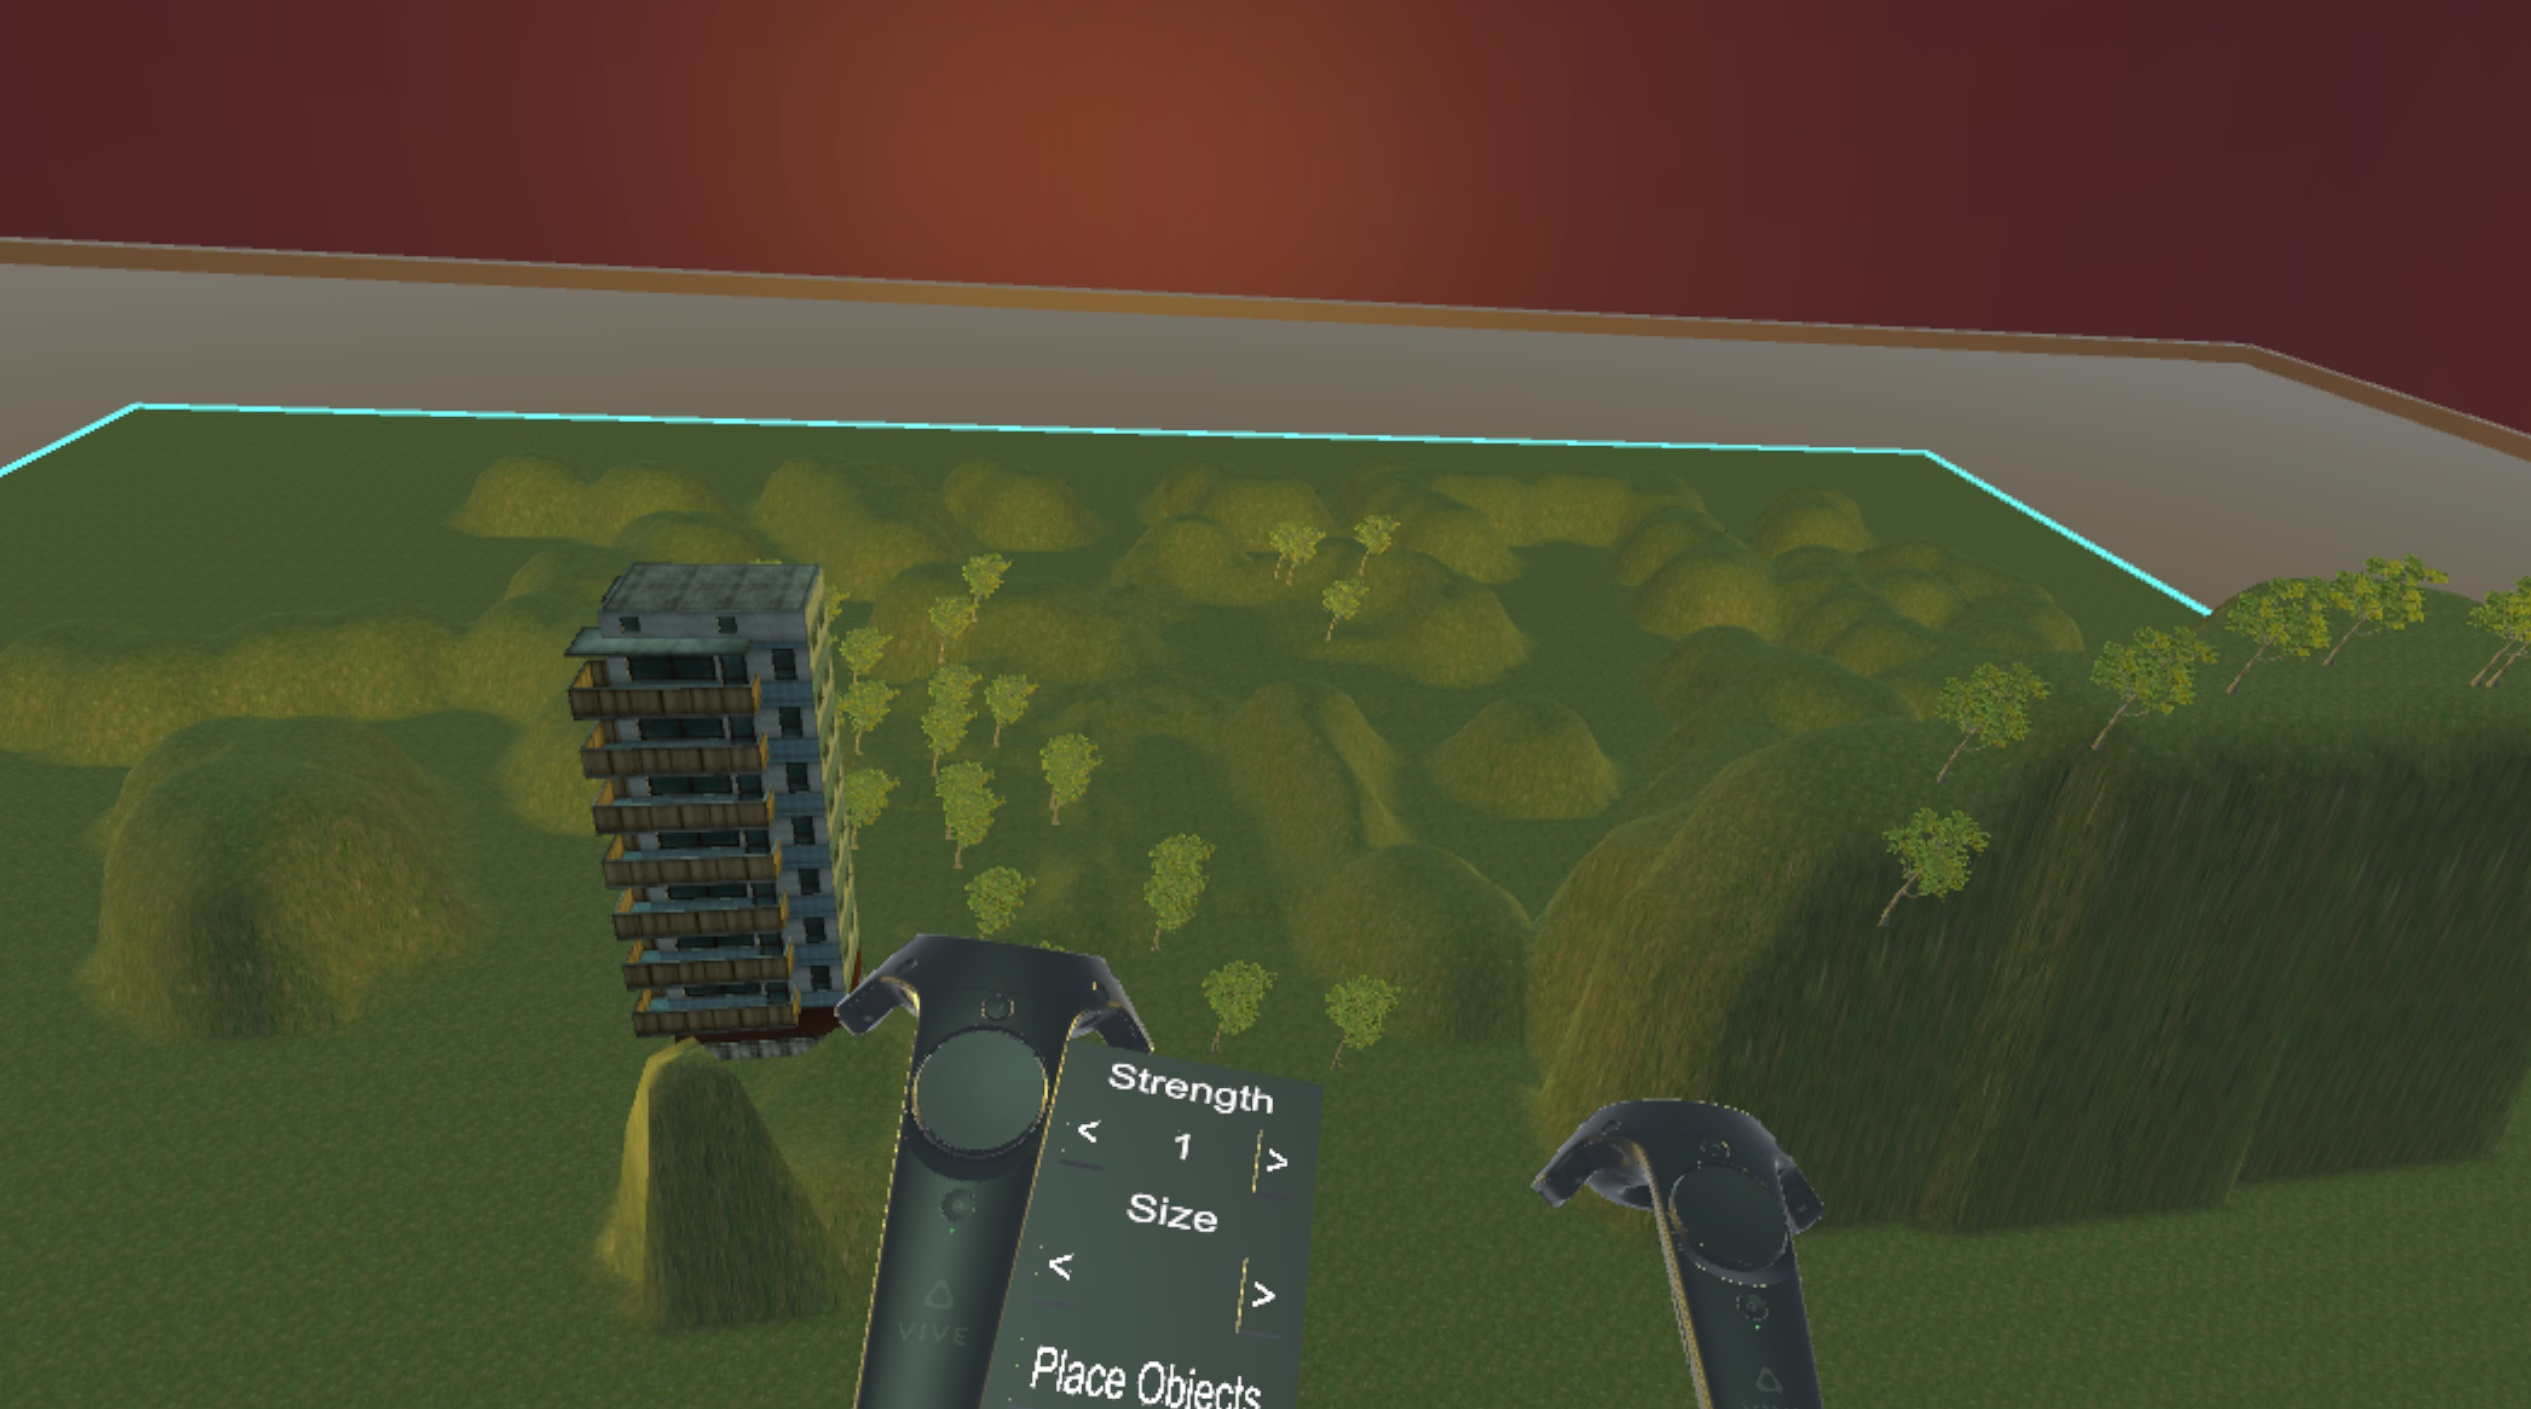
\includegraphics[height=2.3cm,keepaspectratio]{img/screenshots/lobby2.jpg}
    }
    \subfloat[][On-body UI instructions\\in the lobby scene.\label{fig:lobby_screenshot2}]{
        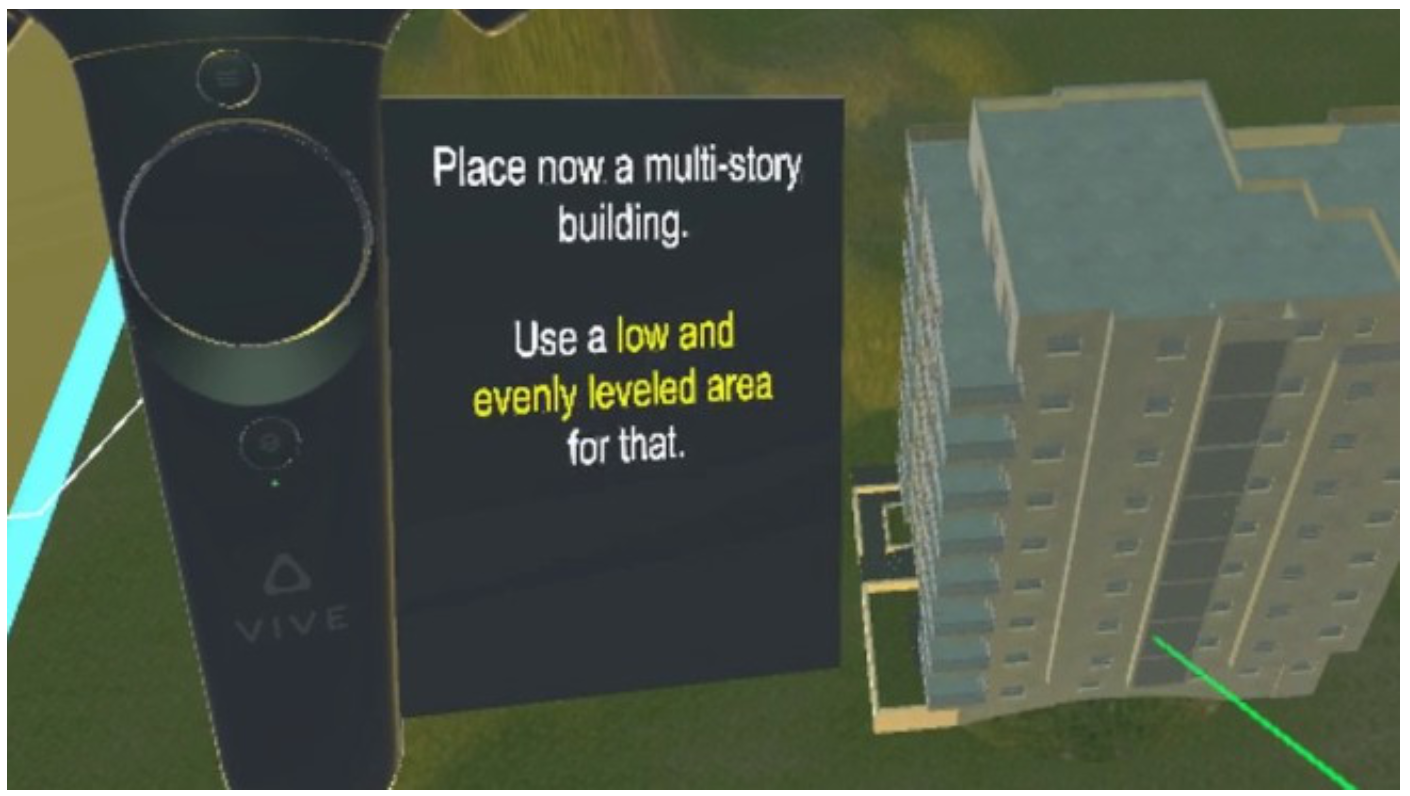
\includegraphics[height=2.3cm,keepaspectratio]{img/screenshots/lobby3.png}
    }
    \subfloat[][Exposure scene with view from a tower building.\label{fig:exposure_screenshot}]{
        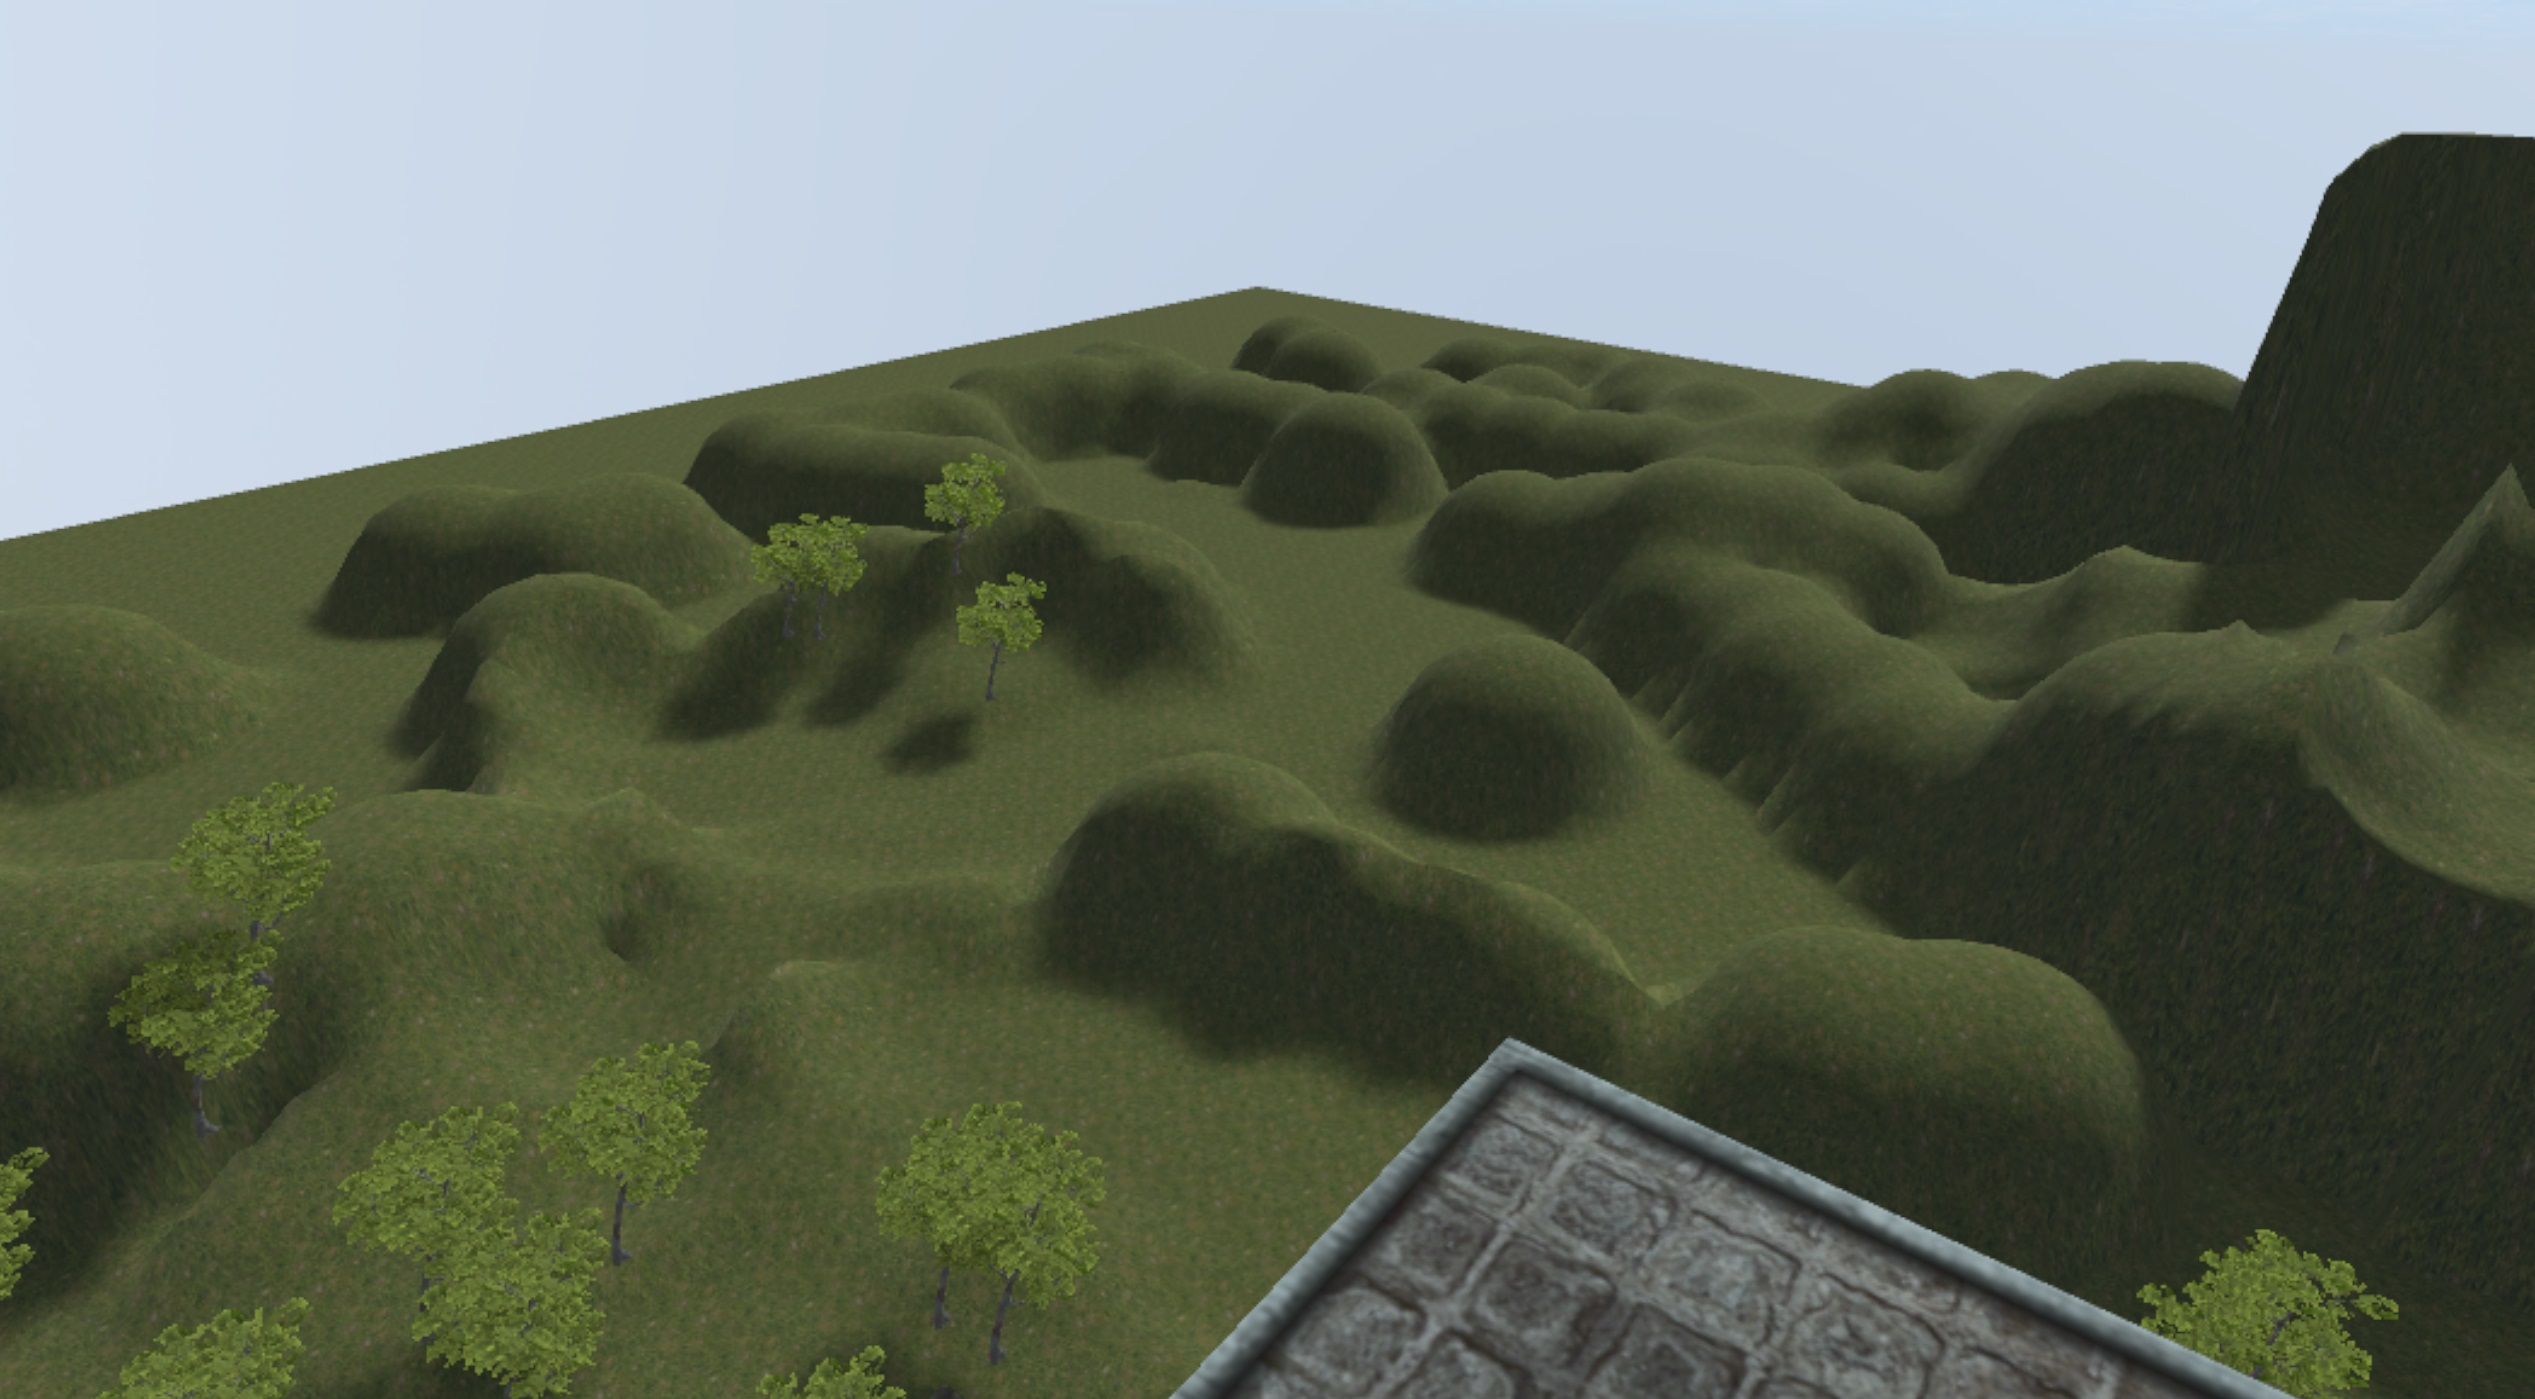
\includegraphics[height=2.3cm,keepaspectratio]{img/screenshots/exposure1.jpg}
    }
    \subfloat[][Questionnaire terminal.\label{fig:invrq1}]{
        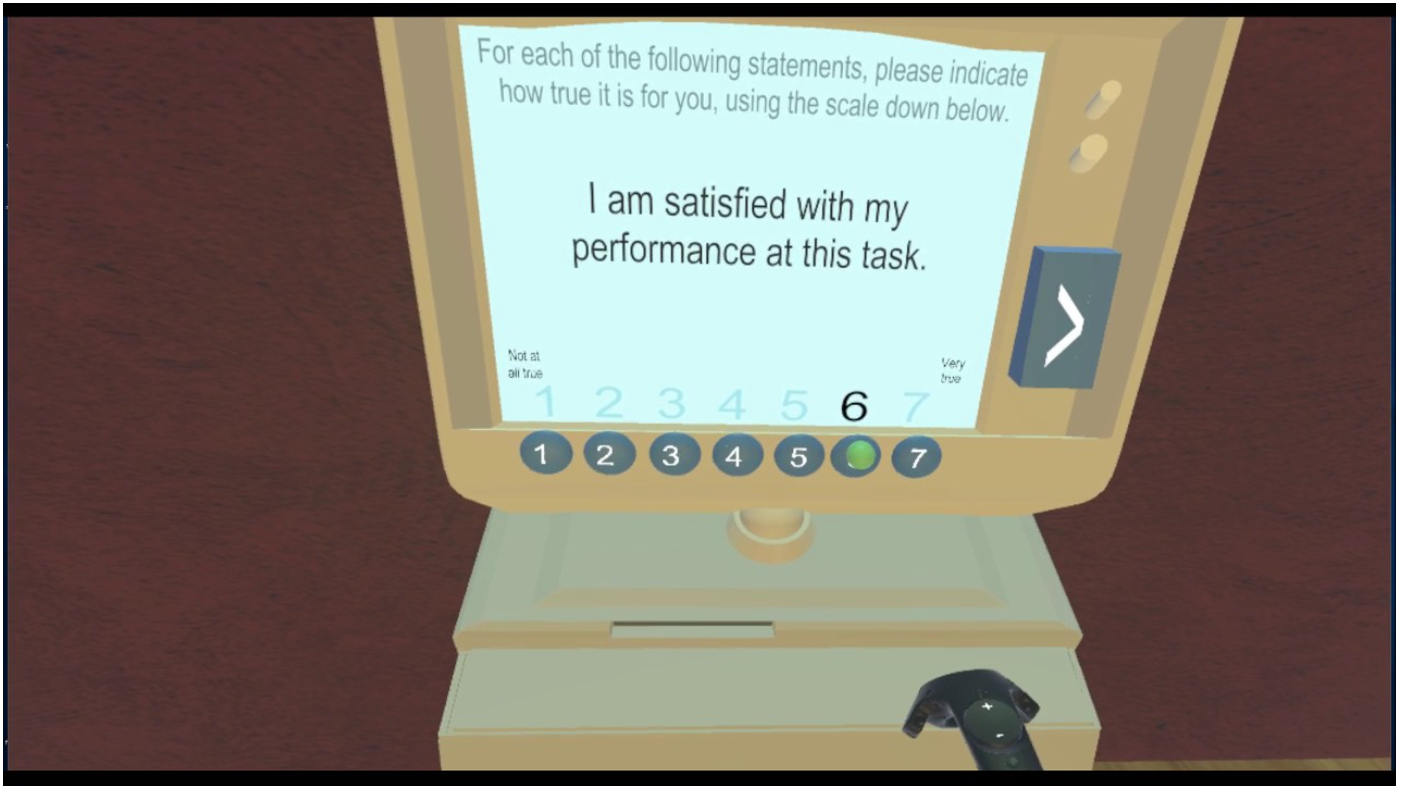
\includegraphics[height=2.3cm,keepaspectratio]{img/screenshots/invrq1.png}
    }
    
    \caption[]{Screenshots of the \ac{VRET} application. \label{fig:screenshots}}
\end{figure*}


\subsection{Requirements \& Design Implications}
Based on the insights from the expert interviews, we discuss how game design patterns can be combined to build a \ac{VRET} system that is  %specifically 
tailored to support therapists who conduct traditional \ac{ET} %exposure therapy 
in treatment of acrophobia. %For that purpose, 
We derive a variety of requirements (\textit{R1}{-}\textit{R5}) that should be taken into account when designing a %applicable 
\ac{VRET} system:
%\newline
% Hallo Marc :-)
% du musst nicht alles als kommentare machen. Wir sehen ja deine Änderungen und gerade bei sowas wie abkürzungen einsetzen ist es ok :-)

% Moin, ja, ist schon Geowhnheit geworden.. Übrigens sollet ihr die Kommentsare dann nachher nochmal saeubern...
% :-)
% Ja das machen wir
%\newline

\paragraph{R1: Motivation} 
% As stated before, motivation to actively seek out therapy to address acrophobia is problematic for a large number of patients. Many people who suffer from this phobia never undergo therapy in the first place or cancel their treatment before habituation is achieved. Therefore, our approach needs to offer motivating elements in order to be an applicable addition to the therapy program. 
From the interviews, we gathered that one key aspect of motivation in the context of \ac{ET} %exposure therapy 
is autonomy. Patients are motivated by pro-actively determining the course of therapy. More precisely, by defining sub-goals and deciding which situations to expose themselves to, they are more engaged in the process which helps them to eventually reach habituation. In summary, a \ac{VRET} application should emphasize the sense of autonomy. This can, for example, be achieved by giving users the opportunity to choose or shape a scenario and the respective tasks.
%\newline

\paragraph{R2: Communication} In line with requirements frequently stated in the literature~\cite{cheek2015,fleming2016}, the communication between therapists and patients was identified to be another crucial element of \ac{ET}%exposure therapy
. Since therapists function as motivators, educators and companions during therapy, a \ac{VRET} system should enable direct communication between them and their patients. This can be achieved by either placing both in the virtual scene (e.g. as avatars~\cite{freeman2018,koller2019}) or at least allowing audio feedback to guide patients through the experience.
%\newline

\paragraph{R3: Scenario habituation} 
% As for the choice of scenarios for the virtual exposure, the therapists provided some crucial insights as well. 
Scenarios should give patients a chance to reach habituation. Therefore, users should have enough time to become familiar with their surroundings. Scenes should come in a variety of different aesthetics in dependence of the respective phobia but are not allowed to be switched too quickly. 
%\newline

\paragraph{R4: Non-distracting tasks} Regarding tasks that provide a meaningful occupation in the virtual scene, the experts proposed some additional requirements. % that should be taken into consideration. 
The typical activity during traditional \ac{ET} %exposure therapy 
involves exposing oneself to the situation in absence of any other specific activities. As a result, tasks in a \ac{VE} should not be distracting, to avoid shifting the focus from the situation to completing some arbitrary task. Notably, this excludes the majority of common game design patterns, which are often built around particular functional challenges and narratives. To enhance motivation, the activities in the \ac{VE} have to be designed with care and should be linked to real-life rewards. 
%\newline

\paragraph{R5: Physiological symptoms} Physiological symptoms are direct results of phobia exposure and help the therapists to monitor the situation and react accordingly. A \ac{VRET} system should be designed in a way that prevents additional symptoms due to technical flaws. Visual stuttering, an unstable frame rate or other visual glitches have to be eliminated. Otherwise, physiological symptoms might be wrongly attributed to the virtual exposure although they emerged on account of technical defects.

% Interlude: Creativity approach in other forms of therapy
%JAN: The following only makes sense to discuss after the specific approach has been introduced...
\begin{comment}
A relatively new movement in psychotherapy that was enormously influential on state-of-the art psychiatry, psychoanalysis, rehabilitation and other therapeutic practices is \textit{art therapy}~\cite{edwards2004}.
This therapy incorporates (playful) creative art making process and is closely related to analytical psychology and psychoanalysis~\cite{edwards2004,hogan2001}.
The created art mediates an externalization process of internal experiences and allows patients to reflect and serves as a frame for the analytic situations~\cite{arttherapy2020, edwards2004}.
Through the art creation process the therapists and patents develop a relationship where conflicts and feelings might find expression~\cite{edwards2004, hogan2001}. 
As this approach incorporates playful experiences in therapy practices this serves as starting point for our game design.
%DIMI: Does it make sense to move art therapy to the BACKGROUND section since we have all RQs in the introduction by now?

* \begin{quote}
    Through integrative methods, art therapy engages the mind, body, and spirit in ways that are distinct from verbal articulation alone. Kinesthetic, sensory, perceptual, and symbolic opportunities invite alternative modes of receptive and expressive communication, which can circumvent the limitations of language. Visual and symbolic expression gives voice to experience, and empowers individual, communal, and societal transformation.
\end{quote}\cite{arttherapy2020}

* \begin{quote}
    Secondly, psychoanalytic theories have been enormously influential in informing the ways in which the therapeutic process is understood. Especially important here are psychoanalytic theories concerning defence mechanisms, play, transference and countertransference phenomena.
\end{quote}~\cite{edwards2004}
* \begin{quote}
    the creative processes and non-verbal communication and be able to provide an environment within which patients or clients feel safe enough to articulate and explore their feelings through the medium of art.
\end{quote}~\cite{edwards2004}
*\begin{quote}
    It is also important that the supervision provided is creative, confidential, and regular, affords opportunities for reflection and is sufficiently flexible to meet the art therapist’s needs at different stages of their career.    
\end{quote}~\cite{edwards2004}

*\begin{quote}
    Kramer’s interests reside not so much in using art or the therapeutic relationship to bring unconscious conflicts into conscious awareness, but in drawing upon the creative process itself as a means of integrating conflicting feelings.
\end{quote}~\cite{edwards2004}
\begin{quote}
    In Kramer’s view, the art therapist’s primary function is to, ‘Assist the process of sublimation, an act of integration and synthesis which is performed by the ego, wherein the peculiar fusion between reality and fantasy, between the unconscious and the conscious, which we call art is reached’ (Kramer in Ulman, 2001: 19).
\end{quote}~\cite{edwards2004}
\end{comment}
%JAN: Wow this was a lot of additional effort to bring in and I sort of triggered it ... so huge apologies, but I think with the recent shift from "creative" to "playful" I would rather suggest to leave this out and instead perhaps simply include a one-sentence pointer down these lines in future work.
% DIMI: No problem. I just wanted to have some options
% - autonomy is key
% - cyber-sickness might by a problem (additional symptom)
% - scenarios aren't allowed to change too quickly
% - virtual reward plan -> achievements in the virtual world linked to real rewards (e.g. collect points in VR and spend them in the real world)
% - habituation should be possible in VR (therefore -> long enough, don't switch levels too rapidly)
% - no distraction, no test of courage
% - "Therefore, to achieve a stronger outcome from gamification, in this thesis it is suggested that not the phase of exposure itself is gamified, but much rather a preparational phase in which the patient builds up a sense of competence and autonomy to increase their feeling of being adequate to the task and accomplish coping with the exposure more easily." (Finke, 2018)
% Discussion: Creativity & Empowerment related 

\section{Game Design for Playful User-Generated Treatment}
\label{sec:game_design}

% - Based on insights from 3) we describe the design and implementation of our tool
%Our interview analysis revealed that game design for acrophobia therapy games requires game elements that are not immersive, should not distract from the exposure task and should not engage for tests of courage. 
%To address the derived requirements for a game-based \ac{VRET} approach, we created a two-step design consisting of a playful design phase and an exposure phase (Figure~\ref{fig:screenshots}). In this section, we describe the concept and implementation of our prototype for \acf{PUT}.
%JAN: Please note that this can be linked to therapist generated or controlled therapy (e.g. in terms of controlling required extent of movement in physiotherapy as in: Marc Herrlich, Jan David Smeddinck, Maria Soliman, and Rainer Malaka. 2017. “Grab-that-there”: Live Direction for Motion-based Games for Health. In Proceedings of the 2017 CHI Conference Extended Abstracts on Human Factors in Computing Systems (CHI EA ’17), 2622–2629. https://doi.org/10.1145/3027063.3053212) ... this could be noted in the discussion and related to future work around "live-control"!?!
%DIMI: \cite{herrlich2017}

%report on a second round of interviews with therapists, where we evaluate and improve our concept. 
%Finally, we present the developed \ac{VRET} prototype and highlight technical details of the implementation.

Our approach splits the \ac{VRET} experience into $2$ distinct phases (Fig.~\ref{fig:screenshots}):
\begin{enumerate*}
    \item The design phase, where participants use a terrain editor in~\ac{VR} to create their exposure (Fig.~\ref{fig:lobby_screenshot} and~\ref{fig:lobby_screenshot2});
    \item The actual exposure phase, in which the participants enter their (self-designed) terrain at full scale (Fig.~\ref{fig:exposure_screenshot})
\end{enumerate*}.

The key of the concept is to allow users to design their exposure in a simulation (top-down view of a miniature map) before they experience it in the exposure at full-scale from a first-person perspective. This approach is in line with recommendations by~\citeauthor{mine2003} who found that user-generated content motivates creativity and self-expression as well as that world-in-miniature models can help conceptualizing the \ac{VE}~\cite{mine2003}.
% JAN: Should there be a note here about whether or not "birds-eye" view of a map constitutes a problem from a perspective of possibly causing fear of height? I would assume that this is a non-issue, similar to looking out of airplanes, but I'm not an expert ... if we don't have a good answer, then perhaps rather leave out for now.
% DIMI: We have answers from the online survey and also from Stefan's interviews that. the miniature terrain shouldn't trigger anxiety. This is also something that we observe in the user study: there are n.s. differences between the conditions on the perception. On the other hand: qualitative feedback from the users highlights that in the \ac{PUT} the users felt the terrain more realistic
This ``sandbox'' approach is designed to foster intrinsic motivation by creating an engagement with -- and a degree of personal relevance of -- the exposure through playful creative action (\textit{R1 Motivation}). Further, the approach empowers patients to adjust the degree of exposure to their specific needs, assess their limits and reflect on the progress, all in collaboration with the therapists. The terrain editor can also be included in the preparatory talks between the therapists and the patients in~\ac{VR} (\textit{R2 Communication}) and help visualize the anxiety-producing stimuli. Since a self-paced \textit{scenario habituation (R3)} was regarded as an important aspect, both phases needed to be designed in a way that gives users enough time and the right interaction options to either shape and customize (design phase) or explore and experience (exposure phase) the virtual scenario. Moreover, for the exposure phase, the interaction needs to be kept simple and focus on allowing the attentive perception of the exposure, explicitly avoiding any potentially \textit{distracting tasks (R4)}. Finally, we opted for a proven consumer-grade~\ac{VR} setup (%namely 
HTC Vive), as the technical setup itself should not cause any additional \textit{physiological symptoms (R5)}.

\begin{comment}
To raise the patients' motivation, we therefore followed concepts from constructivistic learning theories~\cite{papert1991} which propose creativity~\cite{sternberg1998} and exploration~\cite{gee2007} as motivational strategies for playful and engaging learning experience~\cite{duncan2011, ibrahim2009, marone2016, ritterfeld2009,salen2003}. 
This is in line with \textit{Cognitive Theory of Multimedia Learning} which states that active cognitive processes facilitate the learning of new content~\cite{mayer2014}. Hence, interactivity and exploration are essential parts for attentive learning, which arguably is a beneficial state for the support attentively experiencing -- and reflecting upon -- the exposure to virtual heights.
\end{comment}
%JAN: The paragraph above is applicable as there are also close connections between therapeutic approaches and constructivism ... however, it also appears a little out of the blue and opens up several additional possible topics to discuss that are then not really referenced again. If candidates for shortening are needed: this is one.



\subsection{Design Phase}

For the design phase, we created a terrain editor that employed game elements from sandbox games~\cite{projectspark2014,frohlich2018,roo2017} (e.g. Minecraft~\cite{minecraft2009}) and interaction techniques from applications for 3D content creation (e.g. Tilt Brush~\cite{tiltbrush2016}, Blender~\cite{blender1998}), which allow designing own worlds and offer great platforms for customization~\cite{volkmar2020}.
%In VR, users are invited to shape a room-scaled terrain with the controller as sculpting brushes for the terrain. For decoration (e.g. placing buildings, nature or characters in the terrain), users have access to an asset library from a user interface (UI) anchored at the controller of the non-dominant hand.
In the terrain editor, users interact with the~\ac{VE} in tabletop mode using the~\ac{VR} controllers and a commonly used laser pointer metaphor~\cite{jerald2016, laviola2017}.
The terrain is displayed in miniature form situated in a lobby room. To shape the terrain, users press the up and down buttons on the touch pad to raise or lower the terrain respectively. We attached a body-anchored~\cite{alexandrovsky2020, rzayev2019} UI at the controller of the non-dominant hand. From there, users get help or instructions and can select assets (e.g. buildings, nature or characters) to place in the terrain for decoration and personal customization. The asset library consists of $6$ exemplary decoration objects: trees, rocks, grass, bushes, stumps, and wooden cottages. The spawn points can be placed as viewing platforms at different points of height (e.g. on buildings or mountains), which then become entry points in the exposure phase. Therapists can pre-select specific assets for the patients that are convenient for the individual cases. They also have control over the minimum and maximum heights and slopes for the \ac{VRET} as these parameters are most significant for shaping the intensity of the stimulus.

%JAN: How does this relate to a need to be able to realise "realistic" and "personally meaningful" exposure? How was this choice motivated / informed?

\subsection{Exposure Phase}
The exposure phase resembles examples from existing literature (cf.~\cite{emmelkamp2002, powers2008}). To further support a clear focus on the experience, context menus, teleportation and terrain editing tools are disabled. 
%For navigation, we employ the commonly used teleport metaphor~\cite{bowman2004, jerald2016}. 
As a general safety precaution, we implemented a panic button: when pressing all four grip-buttons simultaneously, the screen fades out and users immediately teleport back to the lobby.

We implemented our concept using Unity3D and a HTC Vive with the bundled hand-held controllers as the~\ac{VR} platform. This described approach presents an exemplary instance of an implementation that adheres to the requirements and illustrates a specific response to \acl{RQTwo} in addition to the general requirements discussed above.
%In the following, it will be validated in a user study.



%========================================================
%                      USER STUDY 
%========================================================
\section{Lab-Based User Study}
\label{sec:user_study}

To validate the viability of the requirements and the specific approach described in response to \acl{RQTwo} above and to provide empirical evidence with respect to \acl{RQThree} and \acl{RQFour}, we designed and conducted a user study with non-acrophobic subjects, which investigates the effect of content creation on player experience and height perception.
The study employed the acrophobia \ac{VRET} setup with a playful terrain editor and an exposure to heights in~\ac{VR} as described above. 
%JAN: By the way: one main criticism we will get is : How is this gameful / playful and why were more traditional game elements not considered in the interactions "around" the actual exposure phase ... do we have good answers for that?
%DIMI: 1. the editor is playful because users can decorate the terrain (besides of designing purely the exposure) 2. from the requirement analysis, we know that having traditional game elements (badges, points scores, etc...) are not recommended by the therapists. Therefore we focus primary on the probatory phase. Game elements during the exposure will be addressed in future work?
The study took place in a lab, in which users wore an HTC Vive head-mounted display and could move around in a tracking space of approx. ${2{\times}3}$~\si{\metre}.
The overall size of the virtual landscape at full scale simulates a world of approximately ${40{\times}60}$ \si{\metre} with heights up to \SI{70}{\metre}. However, the surrounding skybox indicates a much larger space and allows for the perception of real-world scale exposure.

Our study included $2$ conditions in a mixed between-subjects setup with repeated-measures. In the first condition (\acl{CPut}), the participants were asked to shape and decorate the terrain with the built-in~\ac{VR} terrain editor.
In the control condition (\acl{CCtrl}), the subjects could only view a pre-defined terrain they were about to enter. Both groups were informed that they would enter the terrain they were viewing or shaping in the second scene. 
We employed subjective self-reports as measures of intrinsic motivation, affect and anxiety.
The assignment to the groups was randomized after balancing for gender.
The study received an ethical approval.

To examine how the playful sandbox-style shaping of the exposure environment affects motivation (\acl{RQThree}) and the perception of height (\acl{RQFour}), we derived the following hypotheses:
%\newline

\textbf{Hypothesis H1:} The activity of shaping terrains provides a measurably higher motivation than viewing a predefined terrain.
%\newline

\textbf{Hypothesis H2}: There is a measurable difference on subjective ratings of anxiety induced by exposure to height between a self-created terrain and a predefined terrain.

\subsection{Participants}
We advertised the study on %the local 
campus, via university mailing lists and through word-of-mouth.
During acquisition, all subjects were pre-screened using the acrophobia questionnaire (AQ)~\cite{cohen1977} to exclude participants showing tendencies for acrophobia. An Anxiety Score of~${>}45.45$ and an Avoidance Score of ~${>}8.67$ were determined as thresholds to exclude subjects from the experiment as it is one standard deviation below the score averages of clinical acrophobics~\cite{cohen1977,antony2005}.
$31$ participants ($25\%$ self-identifying as female) volunteered for our study. The mean age was $24.32$ years ($SD{=}4.32$).
None of the participants showed clinical tendencies for acrophobia (anxiety: \MeanSd{18.87}{11.67}, avoidance: \MeanSd{3,55}{2.36}). $20$ participants experienced~\ac{VR} once; the others had no prior experience with~\ac{VR}. The groups were balanced for gender ($U{=}133.5$, \psig[=]{0.49}), age (\tdf{29}{1.159}, \psig[=]{0.25}), avoidance (\tdf{29}{{\text{-}}1.03}, \psig[=]{0.31}) and anxiety (\tdf{29}{{\text{-}}0.73}, \psig[=]{0.47}).

\subsection{Apparatus}
In our study, we used the prototype as described in Section \ref{sec:game_design} with the following adjustments.
To only allow valid viewpoints in the scene, we restricted the placement of the spawn points to %only 
specific %or 
plausible regions (e.g. viewing platform or rooftops of a building).
Additionally, after completion of the design phase, the following adjustments were applied to the terrain: a) a straight abyss down to the ground level was cut at the view point and b) the surface of each mountaintop was flattened (without notably changing the total height). For the final spawn points, we calculated the position on the spawn platform that was furthest away from the abyss. The rotation was set to look away from the ledge.
To avoid users watching down the ``end of the world'', we restricted the rotation of the buildings so that the viewing platform would always face towards the center of the terrain.
For consistency between the trials in the design phase, we provided only one single circular shaped terraforming brush with a medium strength. 

As we aimed to assess repeated self-reports in \ac{VR}, to avoid breaks in presence~\cite{slater2000} we added questionnaire terminals (see Fig.~\ref{fig:invrq1}) as world-anchored in-VR questionnaires (inVRQs)~\cite{alexandrovsky2020,putze2020}. In the terrain scene, we positioned the questionnaires on the opposite side of the ledge to minimize interference with the exposure when responding.

\subsection{Measurements}
We assessed intrinsic motivation using the \textit{Intrinsic Motivation Inventory} (IMI)~\cite{ryan1982} on the $4$ sub-scales \textit{Interest-Enjoyment}, \textit{Competence}, \textit{Effort-Importance}, and \textit{Tension-Pressure} with $7$-point Likert scales. To get an impression of the participants' emotional state, we applied the \textit{Positive and Negative Affect Scale} (PANAS)~\cite{crawford2004}. PANAS consists of $2$ sub-scales ($10$-items each) that assess positive and negative affect respectively on $5$-item Likert-scales.

\citeauthor{cleworth2012}~\cite{cleworth2012} showed that non-phobic subjects rate the exposure to different heights with different ratings. Therefore, we included subjective measures of anxiety as to validate the effectiveness of the \ac{VE}.
To measure levels of anxiety induced by the exposure to heights, we used the $20$-item \textit{State-Trait-Anxiety-Inventory (STAI)}~\cite{spielberger1983}. STAI contains $2$ sub-scales ($10$ items each) that access the propensity to be anxious (\textit{trait anxiety}) and a temporary anxiety with fluctuating intensity (\textit{state anxiety}).
%JAN: Was this measured only once or twice? I twice: was the trait sub-scale measured twice? Why?
As an additional measure of affliction, we used the \textit{Subjective Units of Distress-Scale} (SUDS)~\cite{antony2005, back2015} -- a single-item visual analog scale ranging from $0$ (no anxiety) to $100$ (highest anxiety).


%To avoid accidental deportations between scenes or spawn points, changing scenes is also accessible from the terminal.
%JAN: Not sure how to interpret that last sentence...
%Our application was running on a high end gaming PC at $90$ fps. 
%JAN: Why highlight 90FPS? If you want to keep this (re: avoid simulator sickness etc.) then also add display resolution, FOV and other technical foundations? Although this should actually be quite clear by saying HTC Vive (and we might get some flak for this being last-gen).

\begin{table*}[t!]
\caption{Mixed-factorial ANOVA for both IMI assesses.}
\resizebox{\textwidth}{!}{%
\begin{tabular}{lcclccclccclccc}
                                        & \acl{CPut}         & \acl{CCtrl}        & \hspace*{0.1em} & \multicolumn{3}{c}{IMI}                                            & \hspace*{0.1em} & \multicolumn{3}{c}{Condition}                                      & \hspace*{0.1em} & \multicolumn{3}{c}{IMI $\times$ Condition}                             \\
\multicolumn{1}{l}{}                    & M (SD)               & M (SD)               &                 & $F_{1,29}$           & p                    & $\eta_p^2$           &                 & $F_{1,29}$           & p                    & $\eta_p^2$           &                 & $F_{1,29}$           & p                    & $\eta_p^2$           \\ \cline{2-3} \cline{5-7} \cline{9-11} \cline{13-15} 
\multicolumn{1}{l|}{Competence}         & 5.18 (0.72)          & 5.22 (0.71)          &                 & 4.12                 &   0.05               & 0.12                 &                 & 0.04                 & 0.85                 & < 0.01               &                 & 3.29                 & 0.08                 & 0.10                 \\
\multicolumn{1}{l|}{Tension-Pressure}   & 2.34 (1.22)          & 2.46 (1.12)          &                 & 32.87                & < 0.01               & 0.53                 &                 & 0.14                 & 0.71                 & < 0.01               &                 & 0.63                 & 0.43                 & 0.02                 \\
\multicolumn{1}{l|}{Effort-Importance}  & 4.69 (1.12)          & 4.55 (1.01)          &                 & 2.25                 & 0.14                 & 0.07                 &                 & 0.15                 & 0.70                 & 0.01                 &                 & 0.53                 & 0.47                 & 0.02                 \\
\multicolumn{1}{l|}{Interest-Enjoyment} & 5.79 (0.97)          & 5.10 (0.89)          &                 & 0.59                 & 0.45                 & 0.02                 &                 & 5.78                 & 0.02                 & 0.17                 &                 & 14.37                & < 0.01               & 0.33                 \\
\end{tabular}%
}
\label{tab:imi_rm_anova}
\end{table*}
\begin{table}[t!]

    \centering
    \caption{One-sample t-tests against a neutral response (4.0) for both IMIs. 
    Top: IMI\textsubscript{1} assessment directly after terrain editing. Bottom: IMI\textsubscript{1} assessment after all 3 exposures.}
    \begin{tabular}{lccc}
    IMI\textsubscript{1}                    & $t_{30}$ & p      & mean diff. \\ \cline{2-4} 
    \multicolumn{1}{l|}{Competence}         & 9.14     & < .001 & 1.06       \\
    \multicolumn{1}{l|}{Tension-Pressure}   & -15.40   & < .001 & \text{-}2.15\\
    \multicolumn{1}{l|}{Effort-Importance}  & 3.09     & < .001 & 0.50       \\
    \multicolumn{1}{l|}{Interest-Enjoyment} & 7.45     & < .001 & 1.41       \\
    \midrule
    IMI\textsubscript{2}                    & $t_{30}$ & p      & mean diff. \\ \cline{2-4} 
    \multicolumn{1}{l|}{Competence}         & 9.88     & < .001 & 1.34       \\
    \multicolumn{1}{l|}{Tension-Pressure}   & -4.73    & < .001 & \text{-}1.05\\
    \multicolumn{1}{l|}{Effort-Importance}  & 3.46     & < .001 & 0.74       \\
    \multicolumn{1}{l|}{Interest-Enjoyment} & 9.07     & < .001 & 1.51       \\
    \end{tabular}%
    \label{tab:imi_one_sample_ttests}
\end{table}{}

\subsection{Procedure and Tasks}
We first informed the participants about the study procedure and gained their consent for participation.
Next, the subjects stated basic demographics and were randomly assigned to one of the conditions (\acl{CPut} or \acl{CCtrl}).
Subsequently, the participants entered the lobby scene. Depending on the conditions, we instructed the subjects differently. In both conditions, they initially entered an empty lobby where we explained the panic switch, navigation and interaction with the inVRQs. After the tutorial, the participants rated their anxiety on the SUDS and we activated the terrain. For \acl{CPut}, we explained the controls of the terrain editor and asked the participants to shape and decorate the landscape to their liking, but with the constraint that the terrain should contain $3$ viewing platforms with different heights each (mid high hill~\SI{30}{\metre}, high hill~\SI{50}{\metre} and a tower building~\SI{70}{\metre}). We chose these heights because all exposures should evoke a sense of notable height at different intensities for convenient subjects (explicitly not suffering from acrophobia).
For \acl{CCtrl}, we pre-designed a terrain that contained the same types of elements available for placement and modification in the other condition. %In order 
To create a meaningful duration for the pre-exposure phase, the subjects were instructed to inspect and memorize the scene. In both conditions, the participants thereby engaged with the terrain for $3{-}5$~\si{\minute}. After \SI{2}{\minute} in, the participants gave a second SUDS rating.
After finishing the editing or memorizing task respectively, the participants completed the IMI as well as a third SUDS and were further instructed to proceed to the next scene (teleport to the next location).

In random order, the participants teleported to all $3$ spawn points and underwent an exposure to heights from each platform. To ensure that the participants were exposed to the heights and did not have their eyes shut, we implemented a secondary task. The participants should throw down a ball and read a series of numbers displayed on the ground when they looked down the pit.
Although the secondary tasks can potentially facilitate an unintended playful experience or a distraction, this or similar tasks have been applied in the experimental setups to encourage participants engaging with the exposure task~\cite{diemer2016, meehan2002, schulz2019}.
%\cite{, } had a similar task
Each trial consisted of the following steps:
%JAN: Huh? I didn't spot this before (sorry; bummer), but doesn't such a task defy everything that was said before about keeping the exposure devoid of game elements!?! THIS SEEMS IMPORTANT! If this was a case, this is arguably more of a game element than the original "sandbox design" phase ... is this a typical element in exposure therapies? If not, this requires careful justification and the entire earlier discussion around phase separation and activities (/avoiding them during exposure) should be reconsidered and possibly adjusted ... not sure how to fix this now, but as is it appears as a logical flaw. This also means that earlier descriptions about "doing nothing" in the exposure phase are wrong!?!
\begin{enumerate*}
    \item Participants pick up a ball and approach the ledge;
    \item They extend their arm over the ledge so the ball is above the abyss;
    \item They let the ball fall and follow it with their sight;
    \item Participants read out numbers shown on the ground floor when the ball hits the ground;
    \item They approach the terminal and rate their anxiety on STAI and SUDS.
\end{enumerate*} We assessed trait anxiety after the first trial. State anxiety was rated after every exposure.
After all $3$ trials, the participants filled out a second IMI and a PANAS and left~\ac{VR}.
We then conducted a semi-structured interview with the participants to gain additional insights about their player experience. On average, participants spent \SI{23.07}{\minute} ($SD{=}3.86$) in~\ac{VR} (\acl{CPut}: \MeanSd{24.2}{4.02}; \acl{CCtrl}: \MeanSd{21.63}{3.24}; \tdf{28.38}{2.14}, \psig[=]{0.02}, Cohen's $d{=}0.76$), with the difference resulting from a varying duration in the first phase. A detailed analysis showed the difference was only significant in the lobby scene (\tdf{11.65}{11.65}, \psig[<]{0.01}, Cohen's $d{=}0.76$)) with \SI{2.07}{\minute} ($SD{=}2.00$) in \acl{CPut} and \SI{3.99}{\minute} ($SD{=}0.36$) in \acl{CCtrl}. The total study duration was about \SI{30}{\minute}.
%JAN: Duration in VR for both phases or only exposure phase? Please be clear ... the difference appears significant (ALWAYS ADD EFFECT SIZE!): what does this mean? Depends on which phases are covered, but sort of conflicts with both "treatments" being the same! So here this speaks for differences in response to \acl{RQThree}/4 and H2?
%DIMI: Effect sizes done. The difference comes only from the design phase (see plot in slack [20.04] 11.47PM
%JAN: Okay ... that is sort of good I think ... however then, I would much rather emphasise that there was no statistically sig. diff in the second (exposure) phase...
%DIMI: mh... die waren in der PUT condition kürzer in der lobby als in Ctrl? Vielleciht wegen, sich das terrain einprägen, haben sie die ganze zeit ausgeschöüft. oh man, bei der studie sind so viele fehler unterlaufen, da hab ich nicht aufgepasst
%========================================================
%                       RESULTS 
%========================================================
\subsection{Results}

\subsubsection*{Intrinsic Motivation}
%\begin{table}[b!]
    \centering
    \caption{Welch t-tests of both IMI measures between the conditions on all subscales. Top: IMI assessment directly after terrain editing. Bottom: IMI assessment after all 3 exposures.}
    \begin{tabular}{lrrrrr}

    \toprule
        IMI1    &     t &    dof &     p &  Cohen's d &  power \\
    \midrule
     Competence &  0.96 &  29.00 &  0.35 &       0.34 &   0.15 \\
       Pressure & \text{-}0.97 &  26.48 &  0.34 &       0.35 &   0.16 \\
         Effort &  0.77 &  28.97 &  0.45 &       0.28 &   0.12 \\
       Interest &  4.08 &  27.65 &  0.00 &       1.47 &   0.98 \\
    %\bottomrule
    \toprule
        IMI2    &       &        &       &            &        \\
    \midrule
     Competence & \text{-}1.12 &  28.90 &  0.27 &       0.40 &   0.19 \\
       Pressure &  0.06 &  28.84 &  0.95 &       0.02 &   0.05 \\
         Effort &  0.04 &  28.90 &  0.97 &       0.01 &   0.05 \\
       Interest &  0.34 &  26.28 &  0.73 &       0.12 &   0.06 \\
    \bottomrule
    \end{tabular}
    \label{tab:imi_ttests}
\end{table}
For all IMI subscales, we conducted mixed-factorial ANOVAs with the respective subscale as a within (repeat-measures) factor and condition as between factor (Fig. ~\ref{fig:imi_combined}). The analysis showed significant differences within subjects only on Tension-Pressure. A Bonferroni-corrected post-hoc t-test confirmed this difference (\tdf{29}{{\text{-}}5.80}, \psig[<]{0.01}, Cohen's $d{=}{\text{-}}1.04$). 
The MF-ANOVA revealed a significant difference between the conditions and an interaction effect on the Interest-Enjoyment subscale. A post-hoc comparison of Interest-Enjoyment with Bonferroni-correction between the \acl{CPut} and \acl{CCtrl} was significant (\tdf{29}{2.40}, \psig[=]{0.02}, Cohen's $d{=}0.43$). There was a significant interaction of \textsc{condition} $\times$ \textsc{Interest-Enjoyment} between \acl{CPut} and \acl{CCtrl} of the first assessment (\tdf{29}{3.90}, \psig[<]{0.01}, Cohen's $d{=}0.70$) as well as between first and second assessment in \acl{CCtrl} (\tdf{29}{{\text{-}}3.17}, \psig[=]{0.02}, Cohen's $d{=}{\text{-}}0.57$).
The results of the MF-ANOVAs are summarized in Table~\ref{tab:imi_rm_anova}.
\begin{figure}[t!]
\centering
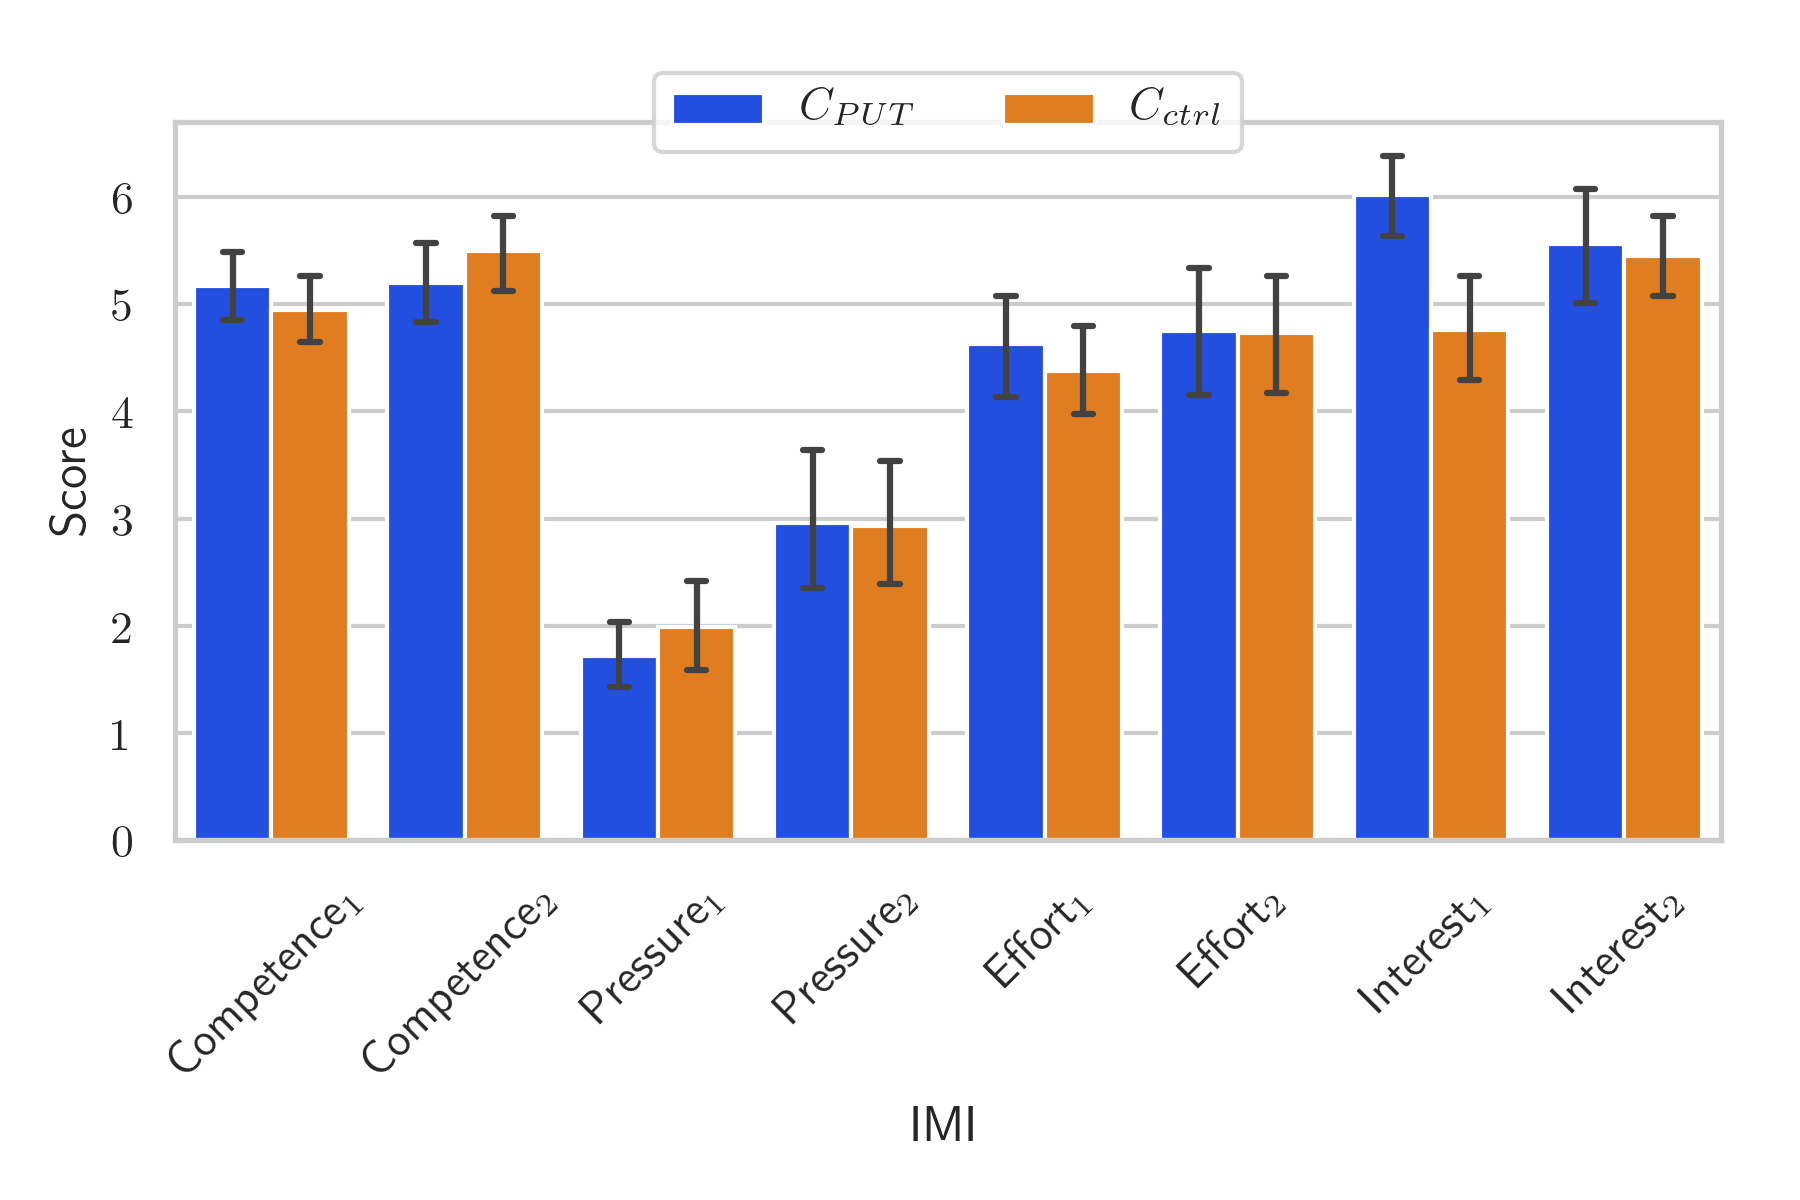
\includegraphics[width=\linewidth,keepaspectratio]{img/plots/imi_combined.png}
\caption[]{Bar plots of both IMI assessments. The whiskers indicate the SD. \label{fig:imi_combined}}
\end{figure}
This indicates that significantly higher motivation potential can be achieved on the Interest-Enjoyment dimension (H1, \acl{RQThree}), while the more functional (competence / effort) and potentially negatively associated (with respect to the application scenario) Tension-Pressure dimension is not likely to differ dramatically (\acl{RQFour}). The lack of differences in the exposure phase and increased Tension-Pressure after the exposure indicate some functioning of the phase as intended (\acl{RQTwo}, \acl{RQFour}).

To determine if the IMI measures deviate from neutral, we performed one-sample t-tests against a neutral score of $4$ (see Table~\ref{tab:imi_one_sample_ttests}). 
The results (all \psig[<]{0.001}) show a positive difference from neutral for Competence, Effort-Importance and Interest-Enjoyment, suggesting that the experience was perceived as challenging, enjoyable and that the participants are willing to invest effort.
Tension-Pressure showed a significant negative difference from midpoint, which can be linked to the exposures not resulting in notable anxiety (as expected with non-acrophobic convenient subjects).

\subsubsection*{Affect and Anxiety}
% \begin{figure}[t!]
% \centering
% 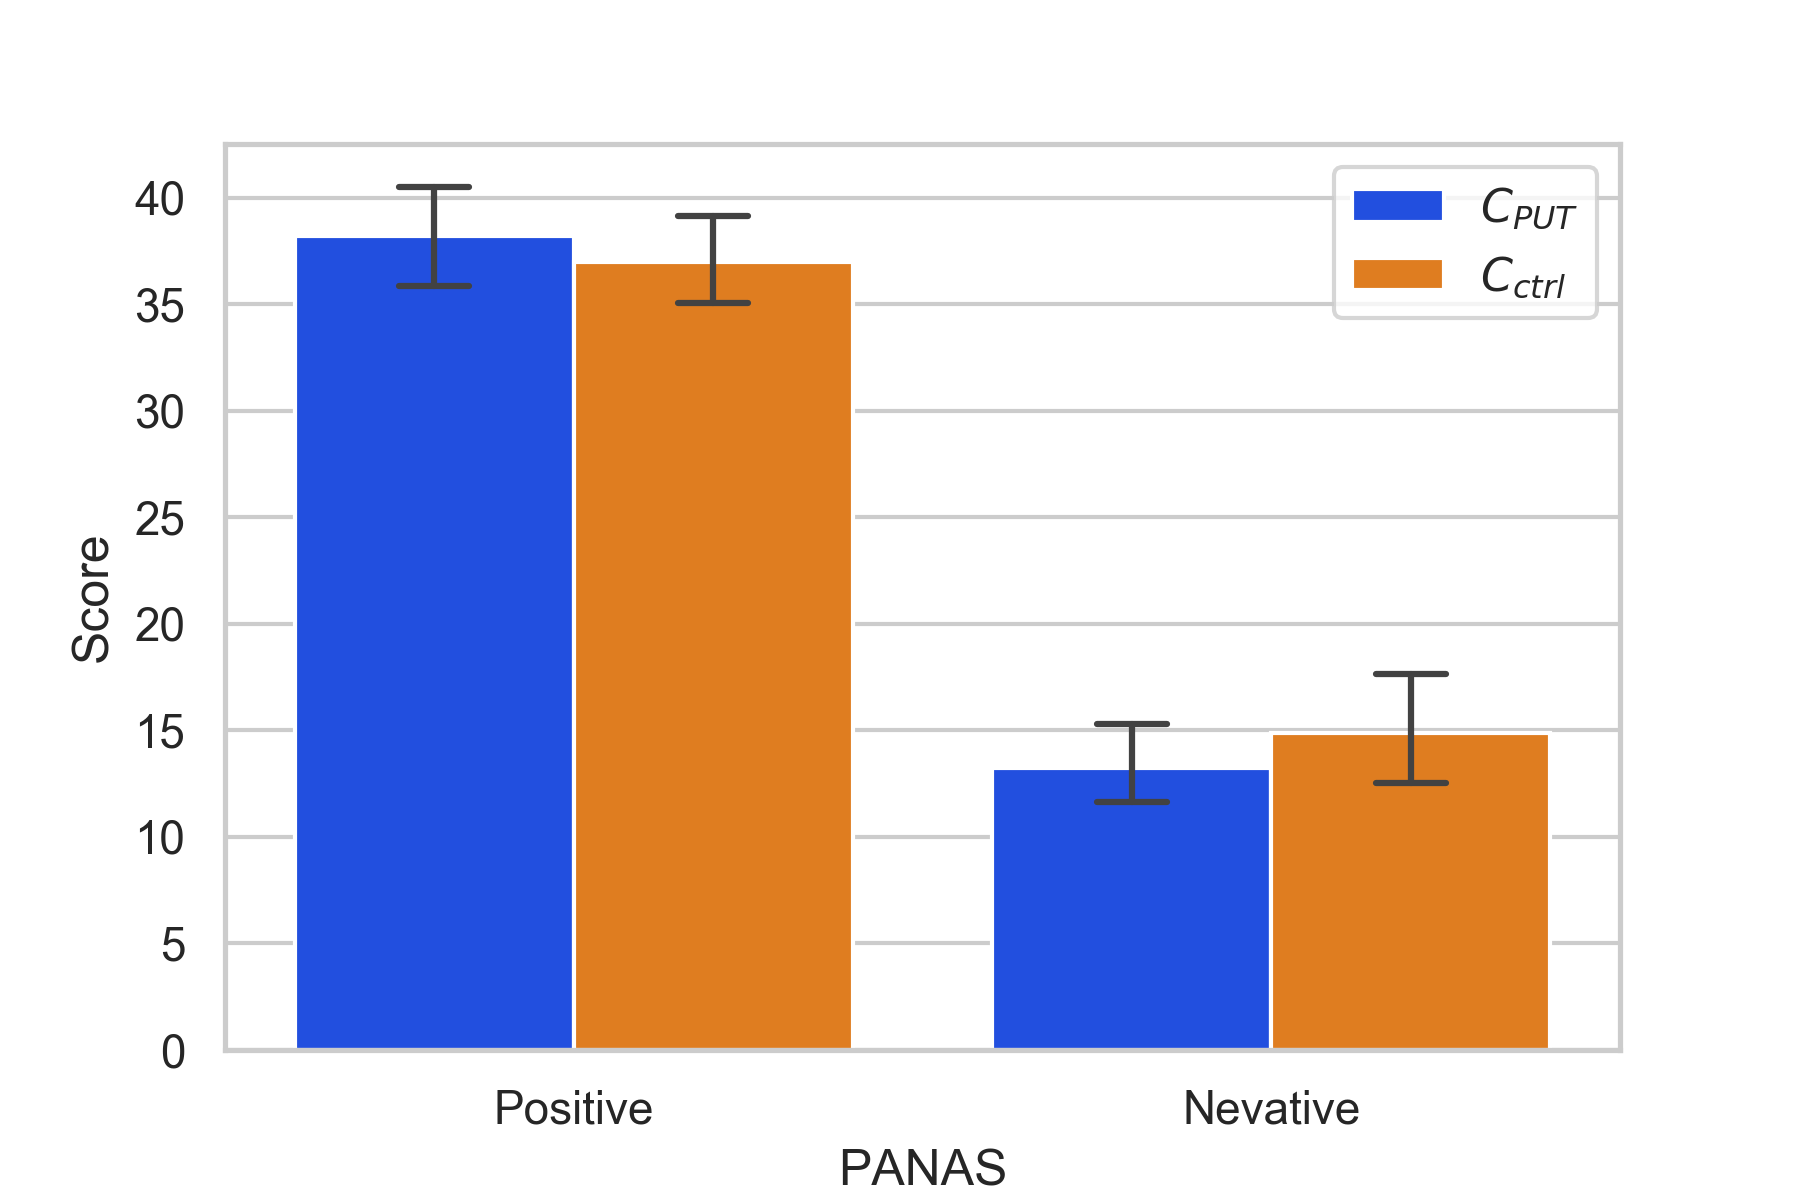
\includegraphics[width=\linewidth,keepaspectratio]{img/plots/panas.png}
% \caption[]{Bar plots of PANAS. The whiskers indicate the SD. \label{fig:panas}}
% \end{figure}

% \begin{figure}[t!]
% \centering
% 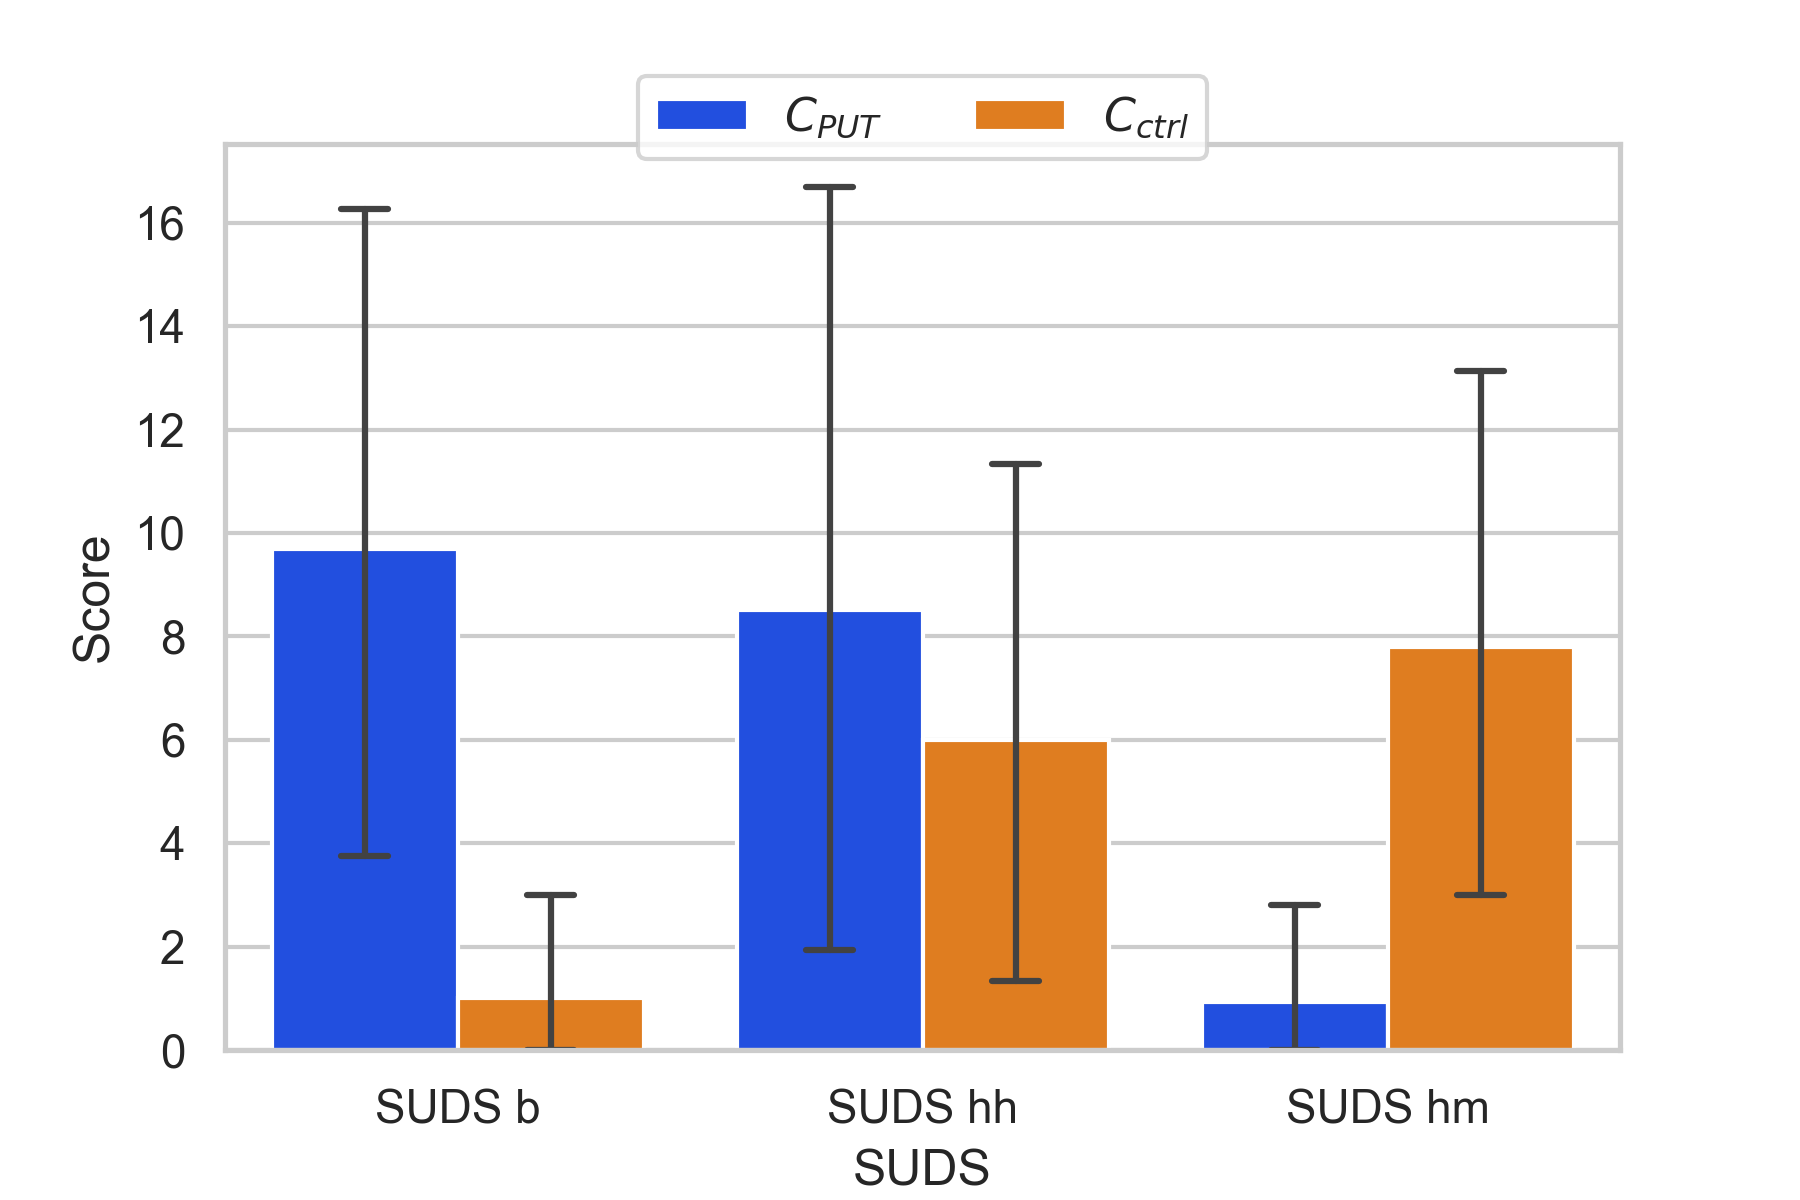
\includegraphics[width=\linewidth,keepaspectratio]{img/plots/suds.png}
% \caption[]{Bar plots of SUDS. The whiskers indicate the SD. \label{fig:suds}}
% \end{figure}





% \begin{figure}[t!]
% \centering
% 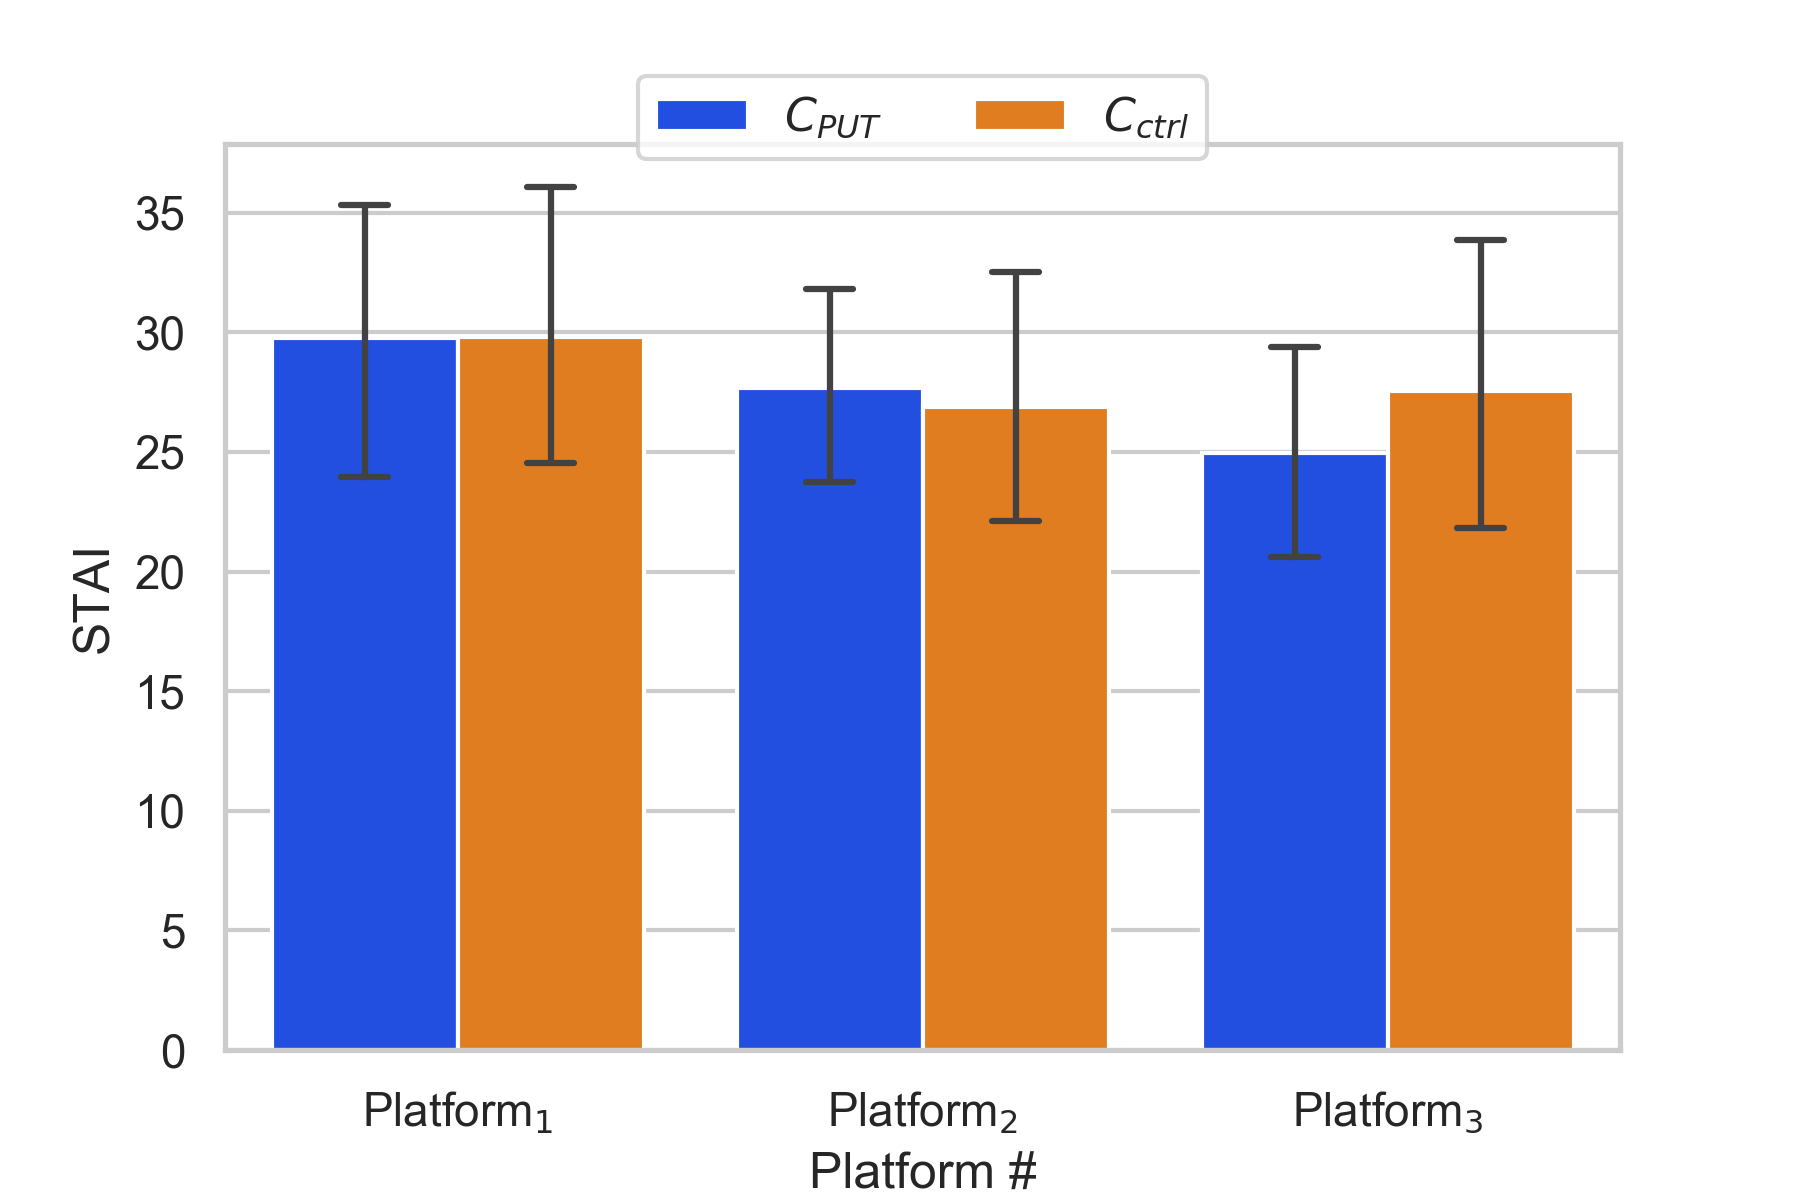
\includegraphics[width=\linewidth,keepaspectratio]{img/plots/stai_order.png}
% \caption[]{Box plots of STAI by order of exposure. \label{fig:stai_order}}
% \end{figure}



We measured affect using PANAS after each exposure task. We conducted independent t-tests to compare the participants' affect between the conditions. Both positive affect (\MeanSd{37.61}{4.39}, \tdf{29}{0.75}, \psig[=]{0.46}) and negative affect (\MeanSd{14.03}{4.55}, \tdf{29}{{-}0.99}, \psig[=]{0.33}) did not differ significantly. This arguably provides further corroborative evidence to comparable exposures (\acl{RQFour}).
For STAI (see Fig.~\ref{fig:stai}) and SUDS as measures of anxiety, we conducted MF-ANOVAs with the $3$ exposures (tower, high, and mid) as within factors and condition as between factor. The results show no significant differences and no interaction effects for both measurements (see Table~\ref{tab:anxiety_anova}).
To investigate how the anxiety evolved over the course of the study, we conducted MF-ANONVAs with anxiety and assessment number (STAI and SUDS) as within factors and condition as between factor. For SUDS, we used the assessment at the end of the first phase as baseline for anxiety. 
%The Greenhouse–Geisser adjustment was used to correct for violations of sphericity of the SUDS measurements.
Both analyses showed significant main effects (SUDS: \fdf{3.34}{67.95}{17.69}, \psig[<]{0.01}, \peta{0.38}, Greenhouse-Geisser corrected $\epsilon{=}0.78$; STAI: \fdf{2}{58}{4.90}, \psig[=]{0.01}, \peta{0.02}) but no significant differences between conditions nor interaction effects. Subsequent post-hoc tests revealed significant differences between platform\textsubscript{1} and platform\textsubscript{3} on both anxiety measures (SUDS: \tdf{30}{2.73}, \psig[=]{0.03} mean diff.${=}3.32$, see Fig.~\ref{fig:suds_order}; STAI: \tdf{30}{2.82}, \psig[=]{0.03} mean diff.${=}3.58$). 
For SUDS, all platforms were significantly more anxiety-inducing than the baseline (platform\textsubscript{1}: \tdf{30}{{\text{-}}5.46}, \psig[<]{0.01}, Cohen's $d{=}{-}0.98$; platform\textsubscript{2}: \tdf{30}{{\text{-}}4.99}, \psig[<]{0.01}, Cohen's $d{=}{-}0.90$; platform\textsubscript{3}: \tdf{30}{{\text{-}}5.54}, \psig[<]{0.01}, Cohen's $d{=}{-}1.00$).
These results indicate that there were perceivable differences between the different levels of exposures in-line with the intended effects (\acl{RQTwo}), while there are no strongly notable differences in the resulting exposure phases between conditions, as intended (\acl{RQFour}, H2\textsubscript{0}).
%The results are depicted in figures~\ref{fig:suds_order} and \ref{fig:stai_order} respectively. 
There was a strong correlation of STAI and Tension-Pressure (Pearson's $r_{29}{=}0.72$, \psig[<]{0.01}) and a medium correlation with Effort-Importance (Pearson's $r_{29}{=}0.43$, \psig[=]{0.02}). This underlines a positive applicability for \ac{ET} %exposure therapy 
 (\acl{RQTwo}, \acl{RQFour}).

\begin{table}[t!]
\caption{Mixed-factorial ANOVA of anxiety measures SUDS and STAI for all 3 exposures.}
% \begin{tabular}{lccclccclcccl}
%                           & \multicolumn{3}{c}{Anxiety}       & \hspace*{0.1em} & \multicolumn{3}{c}{Condition}    & \hspace*{0.1em} & \multicolumn{3}{c}{Anxiety $\times$ Condition} &  \\
%                           & $F_{2, 58}$ & p    & $\eta^2_{p}$ &                 & $F_{1,29}$ & p    & $\eta^2_{p}$ &                 & $F_{2, 58}$      & p        & $\eta^2_{p}$     &  \\ \cline{2-4} \cline{6-8} \cline{10-12}
% \multicolumn{1}{l|}{SUDS} & 0.46        & 0.63 & 0.02         &                 & 0.82       & 0.37 & 0.03         &                 & 3.27             & 0.05     & 0.10             &  \\
% \multicolumn{1}{l|}{STAI} & 0.11        & 0.89 & < 0.01       &                 & < 0.01     & 0.99 & < 0.01       &                 & 2.91             & 0.06     & 0.09             & 
% \end{tabular}%
\centering
\begin{tabular}{lccc}
                                                                 & \multicolumn{1}{l}{} & \multicolumn{1}{l}{SUDS} & \multicolumn{1}{l}{STAI} \\ \cline{2-4} 
\multicolumn{1}{l|}{\multirow{3}{*}{Anxiety}}                    & $F_{2, 58}$          & 0.46                     & 0.11                     \\
\multicolumn{1}{l|}{}                                            & p                    & 0.63                     & 0.89                     \\
\multicolumn{1}{l|}{}                                            & $\eta^2_{p}$         & 0.02                     & < 0.01                   \\ \hline
\multicolumn{1}{l|}{\multirow{3}{*}{Condition}}                  & $F_{1,29}$           & 0.82                     & < 0.01                   \\
\multicolumn{1}{l|}{}                                            & p                    & 0.37                     & 0.99                     \\
\multicolumn{1}{l|}{}                                            & $\eta^2_{p}$         & 0.03                     & < 0.01                   \\ \hline
\multicolumn{1}{l|}{\multirow{3}{*}{Anxiety $\times$ Condition}} & $F_{2, 58}$          & 3.27                     & 2.91                     \\
\multicolumn{1}{l|}{}                                            & p                    & 0.05                     & 0.06                     \\
\multicolumn{1}{l|}{}                                            & $\eta^2_{p}$         & 0.10                     & 0.09                     \\
                                                                 & \multicolumn{1}{l}{} & \multicolumn{1}{l}{}     & \multicolumn{1}{l}{}    
\end{tabular}%

\label{tab:anxiety_anova}
\end{table}
\begin{figure}[t!]
\centering
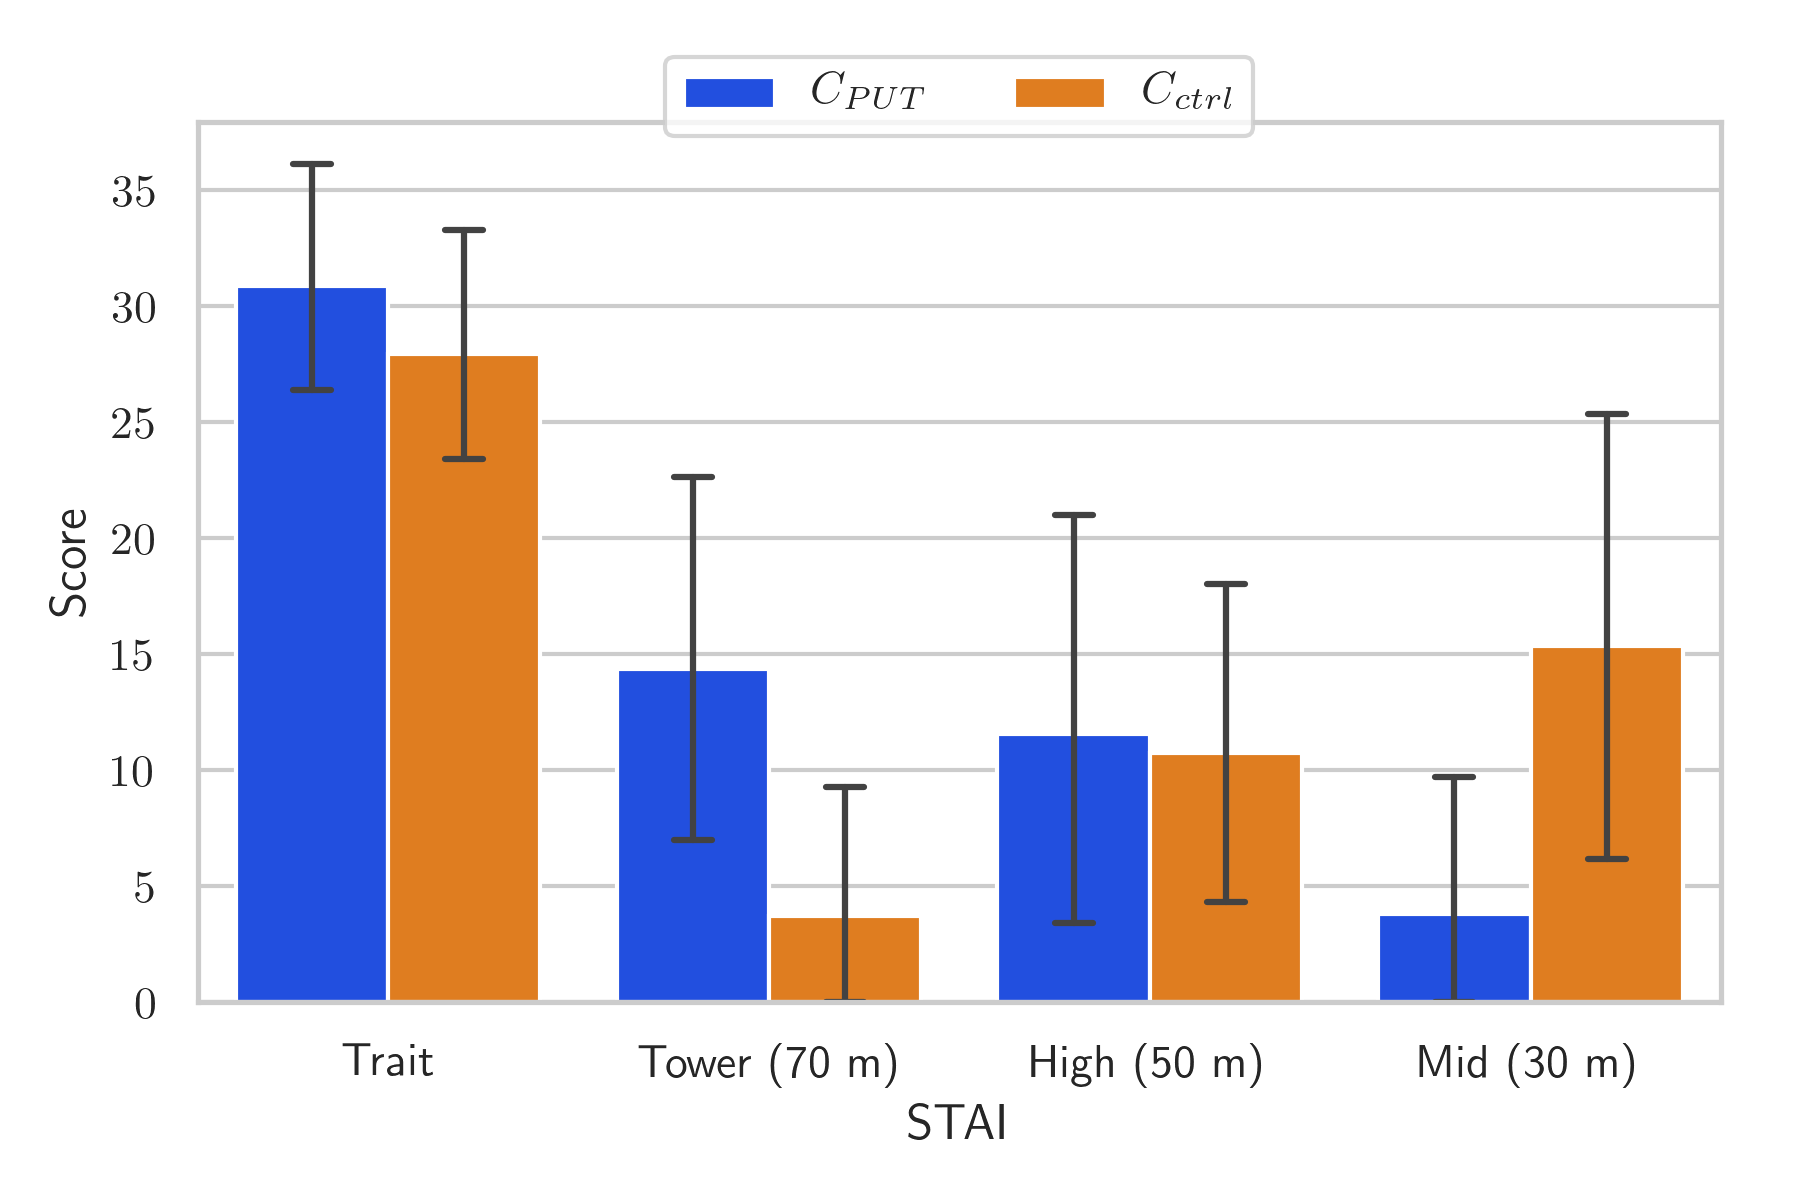
\includegraphics[width=\linewidth,keepaspectratio]{img/plots/stai.png}
\caption[]{Bar plots of STAI. The whiskers indicate the SD. \label{fig:stai}}
\end{figure}


\begin{figure}[t!]
\centering
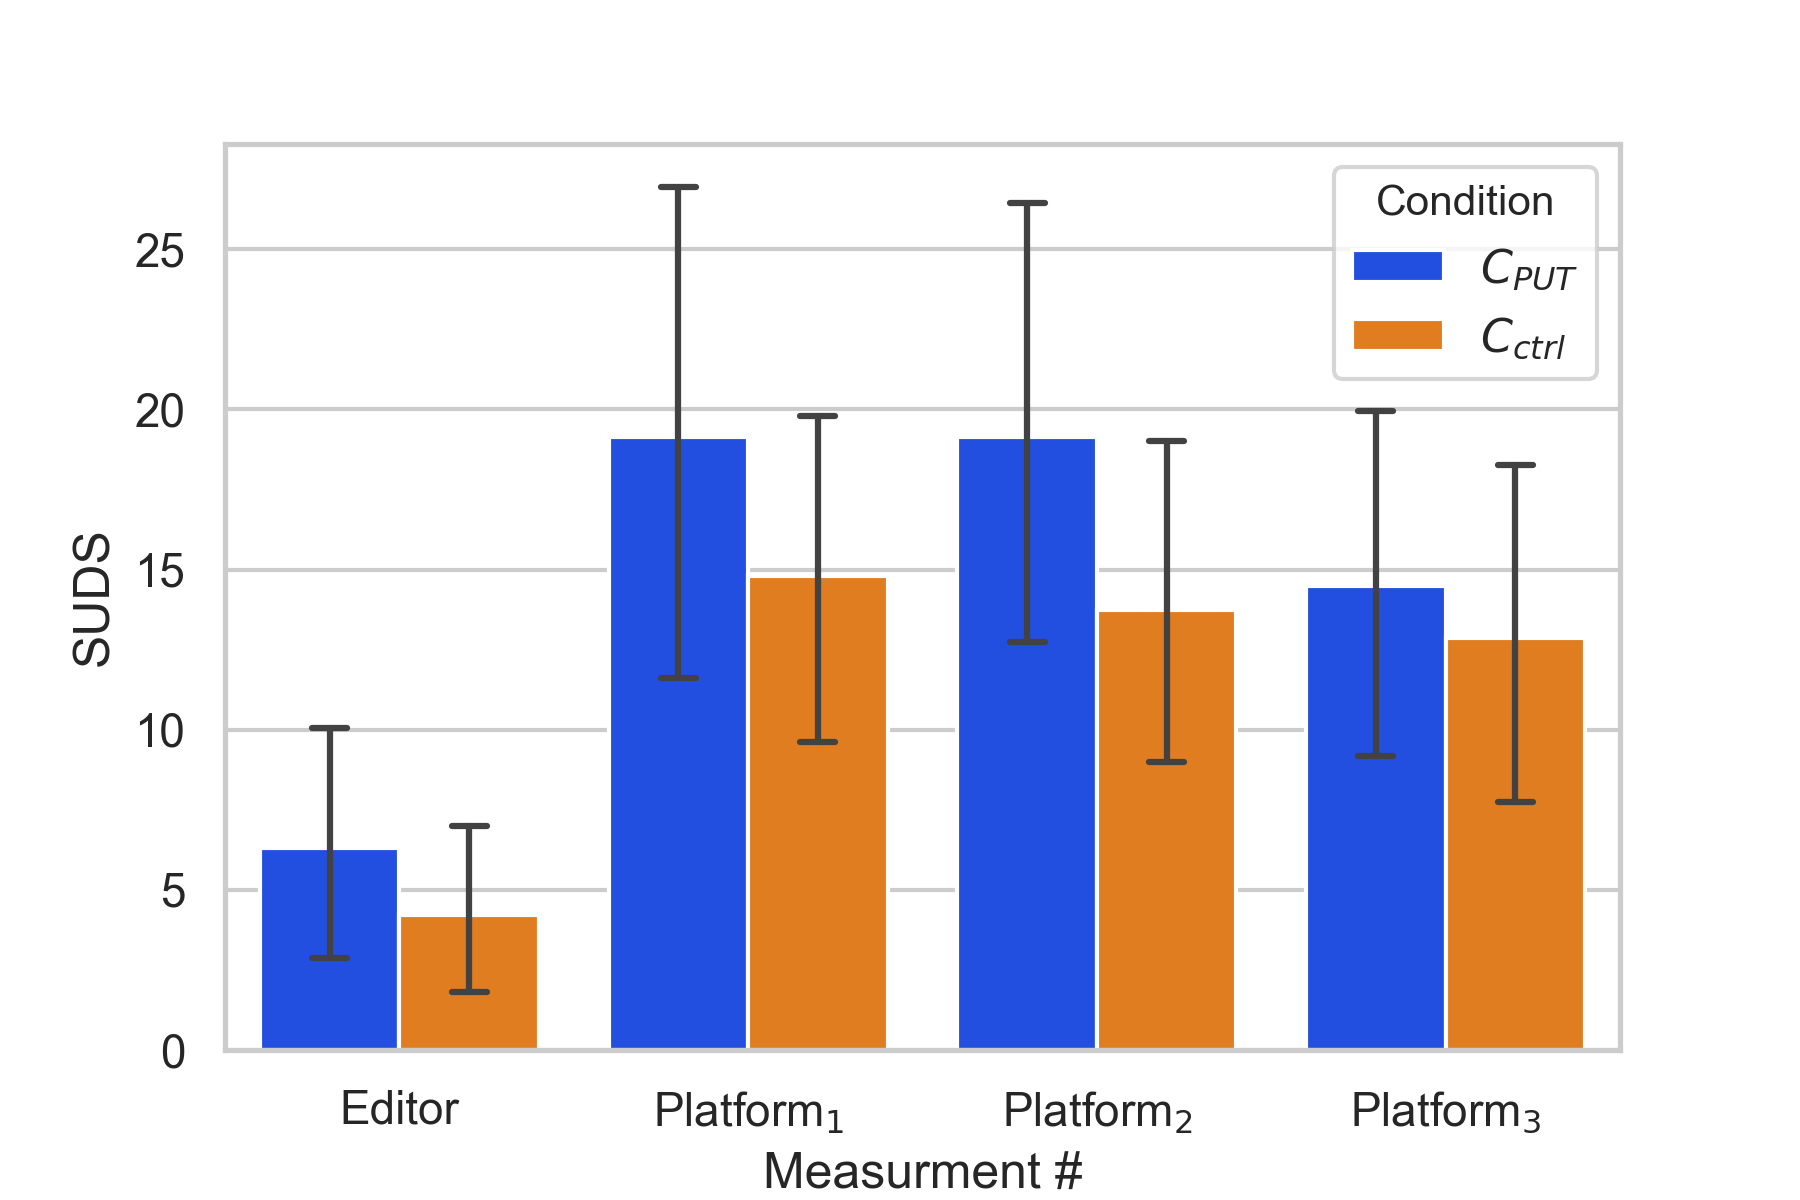
\includegraphics[width=\linewidth,keepaspectratio]{img/plots/suds_order.png}
\caption[]{Bar plots of SUDS by order of exposure. The whiskers indicate the SD. \label{fig:suds_order}}
\end{figure}
\subsubsection*{Qualitative Feedback}
At the end of each session, we asked the participants to comment on their experience and their relationship with the \ac{VE}.
We list paraphrased statements ordered by their frequency:
\begin{enumerate*}
    \item[] ``I felt related to the \ac{VE}'' (\acl{CPut} $15{\times}$, \acl{CCtrl} $1{\times}$),
    \item[] ``The terrain shaping was creative'' (\acl{CPut} $10{\times}$),
    \item[] ``The controls were intuitive" (\acl{CPut} $10{\times}$,\acl{CCtrl} $2{\times}$),
    \item[] ``The experience was interesting or enjoyable'' (\acl{CPut} $9{\times}$, \acl{CCtrl} $6{\times}$),
    \item[] ``I had a vertigo experience when I was looking down" (\acl{CPut} $6{\times}$, \acl{CCtrl} $7{\times}$),
    \item[] ``The environment felt realistic" (\acl{CPut} $6{\times}$,\acl{CCtrl} $0{\times}$),
    \item[] ``I had difficulties with the pointer or teleporter'' (\acl{CPut} $5{\times}$, \acl{CCtrl} $1{\times}$),
    \item[] ``Reading the UI was difficult'' (\acl{CPut} $4{\times}$),
    \item[] ``I would like to have more assets/controls'' (\acl{CPut} $4{\times}$),
    \item[] ``Looking down did not make me anxious'' (\acl{CPut} $1{\times}$, \acl{CCtrl} $7{\times}$),
    \item[] ``There were too many questionnaires'' (\acl{CPut} $1{\times}$, \acl{CCtrl} $0{\times}$),
    \item[] ``I learned something about myself'' (\acl{CPut} $1{\times}$, \acl{CCtrl} $0{\times}$),
    \item[] ``The experience was not interesting or enjoyable'' (\acl{CPut} $0{\times}$, \acl{CCtrl} $6{\times}$),
    \item[] ``I did not feel related to the \ac{VE}'' (\acl{CPut} $0{\times}$, \acl{CCtrl} $4{\times}$),
    \item[] ``The environment felt unrealistic'' (\acl{CPut} $0{\times}$, \acl{CCtrl} $2{\times}$)
\end{enumerate*}.


\subsection{Outcomes}
%- Random assignment was effective: balance for gender, age and trait anxiety
The results show that the \ac{VR}~experience created some sense of anxiety (\acl{RQTwo}), although not to the point of resulting in strong perceived tension or negative affect.
This is supported by the raised SUDSs of all platforms compared to baseline and relatively raised Tension-Pressure of IMI\textsubscript{2} after the exposure.
Also, the significant decay in anxiety both on SUDS and STAI from first to third exposure indicates a habituation which is normal for people without acrophobia. 
The strong correlation of Tension-Pressure and Effort and the anxiety measurements further corroborates these outcomes.
Low negative and high positive PANAS scores as well as positive ratings of IMI show that the experience was generally engaging and positively accepted by the participants (\acl{RQTwo}).

%- H1:
Regarding H1, the higher interest and enjoyment in \acl{CPut} shows that user-generated content can bring up interest. This is further underlined by the qualitative comments which indicate that the process is perceived as creative and supports the forming of a personal \ac{VE}. This is a positive indication for the concept of playful user-generated therapy (\acl{RQThree}).
Moreover, only in \acl{CPut} the subjects stated that the environment felt realistic. Contrary, only in \acl{CCtrl} the participants stated they felt not related, had a low sense of vertigo or lack of realism.
These results show evidence in favor of H1, that user-generated content facilitates aspects of intrinsic motivation.
We observed a significant increase of Interest-Enjoyment in \acl{CCtrl} between IMI\textsubscript{1} and IMI\textsubscript{2}. This results most likely from the non-interactive experience in the lobby. Conversely, we observed a drop in Interest-Enjoyment for \acl{CPut} between IMI\textsubscript{1} and IMI\textsubscript{2} to a level comparable with IMI\textsubscript{2} in \acl{CCtrl}. This can be explained by the simplicity of the experience in the exposure phase and by the participants' low anxiety towards heights.


%- H2:
We could not find conclusive evidence to support H2. 
For anxiety, we only observed differences between the height levels but not between the conditions. These results, together with the  qualitative comments, indicate that the exposure felt realistic and anxiety-inducing without a notable effect of the game elements on the perception of heights. We therefore reject H2 and count this as positive evidence towards the requirement that the game elements should not notably interfere with the exposure (\acl{RQFour}).
However, the results show fluctuations with small effect sizes and a marginal significance. Therefore, it is undue to conclude that there are no effects and these indications require further validation.

With regard to~\acl{RQTwo}, we found that the probatory is a suitable phase of the therapy session to include game elements that do not interfere with the therapy. The self-creation of the phobic stimuli is a welcomed approach for the therapists and allows them to adjust the exposure to the patients' individual needs; a feature that is crucial for effective computer-mediated therapy~\cite{herrlich2017}.
This is in line with the SMART goals~\cite{fenn2013} and with~\citeauthor{thompson2010}'s guidelines and offers opportunities to address the \textit{Goal Setting}, \textit{Problem Solving}, \textit{Motivational Statements} and \textit{Feedback} in game design for therapy~\cite{thompson2010}.
Empowering self-creation mechanics can facilitate creativity~\cite{wang2014,zhang2008} and interest for the therapy and address \citeauthor{malone1980}'s curiosity dimension of educative game design~\cite{malone1980} in contrast to frequently applied elements such as rewards or challenges.
%We further identified, that self-creation of the phobic stimuli is a welcomed approach for the therapists.


\section{Online Survey Expert Evaluation}
\label{sec:online_survey}
%To validate our approach regarding its potential applicability in a real-life therapy scenario, we conducted an online study with practicing therapists. 
To validate our approach regarding its potential applicability in a real-life therapy scenario, we conducted an online study with practicing therapists. For further validation% of the concept
, we included therapists with a wider range of expertise than in the initial interviews. This online survey was not meant to be a final evaluation of a fully functional system but a way to obtain an additional expert perspective on the \ac{PUT} concept.
The survey consisted of a consent form, $12$ questions concerning the proposed game design and $13$ items targeting the respondents' professional background, technical expertise and other demographic data. To illustrate the design approach, the survey contained an introductory text with corresponding images and an embedded video explaining \ac{VRET} in general and demonstrating the \ac{PUT} concept. The $~3$~\si{\minute} long video was compiled from several documentaries from public media on \ac{VRET} and demo clips of~\ac{VR} games and \ac{VRET} applications which corroborate the feasibility of \ac{VRET} as well as a demo of the terrain editor and the exposure phase accompanied by an explanation of \ac{PUT}. For copyright reasons, the video cannot be published.
%JAN: Here one would expect a link to a video figure or an explainer that (why) it will be added later, or why it can't be included. If it can't be shown / included: can you characterise the video in at least a sentence (duration, rough content elements; esp. which bits of the approach discussed above were shown and how)?
%DIMI: Done
After perceiving the material, the therapists filled out the forms which took between $15$ and $20$ minutes. 

\subsection{Participants}
$6$ therapists ($5$ female) filled out the online survey. The group of interviewees included $3$ therapists specialized in depth psychology, $2$ behavioral therapists and $1$ expert in \ac{ET}%exposure therapy
. Their ages ranged from $28$ to $64$ years (\MeanSd{49.33}{13.51}). $5$ experts held an approbation and $1$ a master's degree in psychology. Work experience as a professional therapist was reported to be between $1$ and $31$ years (\MeanSd{11.17}{9.91}). 
All therapists were asked to rate their experience regarding \ac{VR} on a $5$-point Likert-scale ranging from ``No Experience ($1$)'' to ``Expert ($5$)''. On that scale, responses lay between $1$ and $2$ (\MeanSd{1.17}{.37}). 
None of the experts used \ac{VR} in a professional capacity or for entertainment. 
Responses on frequency of utilizing \ac{CBT} methods in therapy included ``never'' ($n{=}1$), ``once a year'' ($n{=}1$), ``multiple times a year'' ($n{=}1$), ``once a week'' ($n{=}1$) and ``multiple times a week ($n{=}2$).
The frequency of treating acrophobia ranged from ``never'' ($n{=}1$) to ``once a year'' ($n{=}1$) and ``multiple times a year'' ($n{=}4$). 

\subsection{Results}
%The online survey consisted of items with fixed responses and open questions. 
%We present the results divided into quantitative and qualitative sub-categories.

\subsubsection*{Quantitative Results}
Regarding applicability in a real-life therapy scenario, the therapists rated the \ac{PUT} design approach on a $5$-point Likert-scale ranging from ``Not Useful'' ($1$) to ``Very Useful'' ($5$). On average, the design received a score of $M{=}3.67$ ($SD{=}.75$) (\acl{RQTwo}). All experts agreed that giving the patients the opportunity to create the environment for later exposure is a valuable approach. The majority of participants ($n{=}5$) stated that separating therapy into $2$ steps (design and exposure phase) may have a positive impact on the course of therapy. The remaining expert expressed it would not affect the therapy. 
Regarding the influence of the patient's contact with the scaled-down miniature terrain (\acl{RQFour}), the experts reported that it may lead to positive effects ($n{=}4$) or no effects ($n{=}2$). 
Since non-distracting tasks were identified to be one core requirement of \ac{VRET} design, we asked the experts if the design phase may distract from the actual exposure (scale ranging from ``No Distraction''  ($1$) to ``Full Distraction'' ($5$). 
This item received an assessment of $M{=}2.00$ ($SD{=}1.15$) (\acl{RQFour}). 
Regarding communication between therapists and patients, $4$ therapists would like to accompany their patients during the design phase, whereas the remaining $2$ experts stated this would not be necessary. 

\subsubsection*{Qualitative Feedback}
$2$ experts stated that a playful approach would be beneficial in preparation to real-life exposure as the situation itself would not be perceived to be as terrifying as in the real world. However, since the virtual representation of phobia-inducing stimuli lacks in realism, $3$ experts explicitly stated that it should not replace real exposure. Additionally, $2$ experts pointed out that communication should be enabled by the system whereas $1$ therapist wished to enter the virtual world along with the patient. $1$ expert reported that \ac{PUT} may lead to a higher sense of control (\acl{RQThree}) and perceived self-efficacy. Another therapist reinforced this assessment by stating that \ac{PUT} design could give patients a sense of security. As a suggestion for future development, $1$ therapist proposed the idea of exposing patients to virtual scenes that were not created by them in later stages of therapy.

% TODO: comments from therapists
% Both interviewees considered the approach as beneficial and motivating for the course of the therapy.
% The interviews highlighted several aspects to consider when designing playful \ac{VRET} applications.
% The gamified process must not give the impression that there are varying levels of difficulty and that they could choose to start with an easy challenge, as this would be counterproductive to what is taught to the patients in preparation for the exposure.
% Overall though, the idea was met with positive reactions, receiving confirmation that the concept of using a gamified creation tool may indeed increase motivation by not only evoking feelings of autonomy and self-efficacy but also because the tool would be a way to signify that the needs of each individual patient are considered by the therapist.
% This could be a way to increase the patient-therapist alliance which has been unexplored so far in previous research. In the interviews however it was confirmed that it is one of the most important aspects when trying to secure the motivation of the patient to see the therapy through.




% From e thematic analysis we clustered the responses in $13$ categories. We present the results aggregated according to the categories.

% \paragraph{Conditions and Aspects for Successful Exposure Therapy}
% The willingness to participate and complete exposure depends greatly on the trust and belief in the competence of the therapist (C3,7)(C4,5)

% \paragraph{Common Scenarios for Acrophobia Treatment}
% For acrophobia specifically, it is suggested to use high towers or a viewing platform that allows to look far and down (C5,1)(C5,2). In a more general sense, especially for people with acrophobia, it would be more simple situations that cannot be fled easily, like festivals, masses of people and train stations (C5,4). The same applies to means of transport that don't stop very often and are therefore inescapable (C5,3).

% \paragraph{Feedback on the Suggested Game Design}

% Both therapists agree on Virtual Reality as a means to recreate immersive stimuli for exposure therapy is in general positively received and considered useful (C7,1)(C7,9).

% One more aspect that was regarded positively was how it would positively influence the cooperation between therapist and patient. First of all, it could help the therapist to identify and diagnose further attributes of their disorder during the process of creating their own stimulus of fear (C7,5). If the therapist is able to contribute before or during those sessions, it could be secured that they can direct and help with their professional competence to help create custom tailored stimuli that are effective for exposure therapy (C7,4). It could help improve the willingness of the patient as some of them do wish to approach situations that are known to them (C7,12).

% Overall, the impression was gained that based on these facts, the motivation could be really improved through the process of creating their own stimulus in Virtual Reality (C7,14).

% It was also expressed to be cautious though. If the choice of less or more intense stimuli would imply that there was a gradual increase in difficulty and that more intense stimuli are only endurable by having gained a competence for it, it may backfire as more fear shouldn't mean more danger (C8,4)(C8,5). It should not support the choice to choose something more safe than something more intimidating (C8,6).

% Also concerns were expressed that the patient should not be affected by vertigo induced by the virtual reality system (C8,1).


\section{Discussion}
\label{sec:discussion}
With regard to \acl{RQOne}, we identified $5$ considerations for \ac{VRET} game design. 
For an auspicious computer-mediated \ac{ET}%exposure therapy
, patients should have control over the course of therapy by defining tasks, goals and situations themselves (R1). \ac{VRET} should allow for direct communication between therapists and their patients during exposure (R2). Scenarios should come in rich variety but leave patients enough time to get accustomed to and %thus, ultimately 
reach habituation (R3). As for potential in-game tasks, they should be linked to real-life rewards but not be too distracting from the exposure or be perceived as tests of courage (R4). The system itself should not cause any additional physiological symptoms that might be wrongly attributed to exposure (R5). Most of these requirements are in line with the SMART goals
~\cite{fenn2013} and  existing frameworks on game design for interventions (cf.~\cite{coyle2007, fleming2017,thompson2010}).
However, we found the combination of motivating (R1) and non-distracting game design (R4) a specific requirement for \ac{VRET} that is rarely discussed in the literature on games for change.
%To close this gap, we developed and evaluated \acf{PUT} as a two-step design pattern \ac{VRET}. 
%Our approach builds on concepts from constructivistic learning theories~\cite{papert1991}  and art therapy~\cite{edwards2004}, which propose creative enaction and self-empowerment at its core.
% DIMI: Please help with wording!!!!
%* To investigate the practicability of \ac{PUT}, we conducted a user study that investigated the effect of self-created anxiety stimuli on player experience and height perception as well as an online survey with practicing therapists who rated and discussed the approach (\acl{RQTwo}). 
The outcomes of the user study show evidence that self-generated anxiety stimuli can raise the intrinsic motivation for a simple task (\acl{RQThree}, H1) while not interfering with the sense of anxiety (\acl{RQFour}, H2\textsubscript{0}) and thus, our design approach fulfills R1 and R4 explicitly.
The experts involved in the online survey gave an overall positive assessment of \ac{PUT} design in terms of applicability in a real therapy scenario (\acl{RQTwo}). A minority of the therapists was concerned that the patients would avoid challenging themselves.
Most therapists acknowledged the \ac{PUT} concept to be applicable, to have a positive effect on the motivation (\acl{RQThree}) and not being too distracting (\acl{RQFour}).
% Marc: Why no specific numbers but "most", "minority", etc?
Moreover, the survey identified potential for improvements for future iterations such as a communication interface between the therapists and the patients. The experts emphasized that communication between therapists and patients is crucial and should be anchored deeply in the design. They highlighted that~\ac{VRET} should be considered as an addition but not as a replacement for conventional~\ac{ET}.
These triangulated results corroborate that \ac{PUT} appears to be a viable concept that warrants further development and study.
%* Experts: However, it should not replace real exposure. Concept could be improved by fostering communication between patients and therapists and to allow entering scenes not created by the patients themselves.

\subsection{Limitations and Future Work}
Empirical user studies with phobics are ethically problematic, since they require experienced support in case of a panic. Therefore, this early-stage research evaluated the approach with convenient subjects. 
However, \citeauthor{robillard2003}~\cite{robillard2003} compared emotional reactions of phobics and non-phobics to different phobias in~\ac{VR} and showed that both groups react to phobic stimuli similarly but to a different degree; with phobics being affected by the \ac{VE} stronger. Interestingly, the authors found no differences in the perception of game elements. This shows evidence that evaluation of game design for exposure-based~\ac{VR} with non-phobics should generalize to phobics as well and may be transferred to other phobias. 
According to~\citeauthor{coyle2007}~\cite{coyle2007}, this work is situated in the first phase of the development cycle. In future work, we aim to investigate \ac{PUT} with afflicted subjects under the supervision of therapists.
In the study, we did not assess autonomy since the study was conducted with convenient subjects and therefore, we did not expect a raise on autonomy, as no deregulation compared to traditional \ac{ET} %exposure therapy 
would be notable to the subjects.
However, literature on motivation shows that user-generated content can raise the sense of autonomy and competence~\cite{ryan2000,wang2014,zhang2008} and that creativity is linked to self-empowerment~\cite{sun2012}. As the study was mainly concerned with the interference of game design, height perception and intrinsic motivation, assessment of autonomy was beyond scope. This should, however, be addressed explicitly in future work with phobic patients and~\ac{SDT}. 
%The three dimensions of competence, autonomy and relatedness form an interesting potential interface to discuss motivation, as it has been successfully employed both in the context of therapy and game design.
Further, the subjective ratings on anxiety (SUDS and STAI) show high variances that are likely attributed to low sensitivity towards heights. Although this work is based on validated measurements, future work should consider physiological measures of anxiety such as heart rate or galvanic skin response for clearer and more reliable data.

As fear generally embodies avoidance, it is difficult to create an intrinsic motivation to coping with one's phobias. Thus, presenting anxiety inducing stimuli in an enjoyable way is a challenging demand for game design.
%This work is a first attempt to investigate the design space for \ac{VRET} games. 
Our research shows that game design for non-intrusive playful experiences is rarely explored in the literature and requires further attention. Likewise, further traditional game elements could be employed, especially in the design phase, as well as game mechanics that may contribute positively to the therapeutic potential of the exposure phase, e.g. around vertigo experiences or emotional challenges associated with phobias. Both are underexplored in the literature and should be considered in future research on \ac{VRET} games.


%========================================================
%                      CONCLUSION 
%========================================================
\section{Conclusion}
\label{sec:conclusion}
% \acl{RQOne} - interviews, requirements
%In this paper, 
We presented a novel game design approach for~\ac{VR} exposure therapy: \acf{PUT}. We investigated this concept with a multi-angled approach: a requirement analysis, the implementation of a~\ac{VR}-based game, a user study with convenient subjects, and an online survey with a distinct group of therapists.
The requirement analysis revealed that \ac{VRET} is considered to be a useful addition to conventional therapy and that \ac{VRET} game design demands specific considerations, which are rarely addressed in the literature. The requirements led to the \ac{PUT} design approach that separates \ac{ET} %exposure therapy 
in~\ac{VR} into design and exposure phases. Our two validation studies with the~\ac{VR} game show that \ac{PUT} is well applicable. In particular, the user study reveals that the users' content creation leads to increased interest and enjoyment without notably influencing affective measures during the exposure session. The positive indications with convenient subjects also suggest that further study and validation in an applied therapeutic context appear warranted.
%This work can help researchers and practitioners designing motivational and playful experiences in the context of exposure therapy in~\ac{VR}. 

% A game-based approach is attributed with the potential to strengthen motivation and autonomy as important factors for successful therapy. 

%Results from the study indicate that \ac{PUT} successfully evokes a sense of anxiety whilst keeping the distraction from exposure to a minimum. In comparison to traditional VRET, the \ac{PUT} approach lead to a higher sense of interest and enjoyment for the respective users. 


%JAN: Das kann man hier kürzer halten ... ist ja alles schon gesagt ...
%DIMI: conclusion ist grad kraut und rüben, ich hatte grad damit mehr oder weniger angefangen
%JAN: okay ... wird schon noch werden ... ich muss jetzt schlafen und bin dann auch erst einmal durch ... ist ein spannendes paper mit vielen tollen aspekten ... ich hoffe, dass das mit dem kuerzen noch klappt und wenn die CHI Play es nicht mag, dann kommt das mit revisions sicher wo anders unter!

%Dimi: vielen, vielen dank jan! ja das paper ist recht spannend habt aber auch tiefe löcher. ja das bekommt man sicher irgendwo unter. MUC niveau ist es alle mal :-D 
%DIMI:schaust du morgen nochmal drauf?
%JAN: Schaffe ich leider realistisch betrachtet nicht mehr, sorry ... zu viele brennende Baustellen
%DIMI: Kein problem. kann ich auch verstehen. Das wird schon. wir haben ja noch Tanja
%DIMI: Also danke dir nochmal. ach eine sache noch. bei VRestionnaires wolltest du hinten stehen, wie ist das hier?




%JAN: CONSIDER MOVING THE LINE ABOVE TO THE CONCLUSION...

% our work shows that \ac{VRET} games demand specific requirements that are not applicable to traditional game design approaches such as scoring systems or badges etc....

\begin{comment}
Finally, our validation studies of a prototype implementation (a lab-based study with users and an online survey with experts) show that the \ac{PUT} approach is well applicable. In particular, the analysis of the user study reveals that the user generated content phase leads to increased interest and enjoyment without notably influencing affective measures during the exposure session compared to a baseline condition without the \ac{PUT} element.
%JAN: CONSIDER MOVING THE LINE ABOVE TO THE CONCLUSION...
\end{comment}








%%
%% The acknowledgments section is defined using the "acks" environment
%% (and NOT an unnumbered section). This ensures the proper
%% identification of the section in the article metadata, and the
%% consistent spelling of the heading.
\begin{acks}
This project was partially funded by the project \textit{Scalable Pervasive Health Environments} of the German Research Foundation (DFG) as part of the SPP 2199.
\end{acks}

%%
%% The next two lines define the bibliography style to be used, and
%% the bibliography file.
\bibliographystyle{ACM-Reference-Format}
\bibliography{FearOfHeightsVR}

%%
%% If your work has an appendix, this is the place to put it.
\appendix



\end{document}
\endinput
%%
%% End of file `sample-sigchi.tex'.
